\documentclass[mathserif]{beamer}
\usetheme[secheader]{pecostalk}
\graphicspath{{figs/}}             
\usepackage{pict2e}
\usepackage{subfig}
 
\newcommand{\pp}[2]{\frac{\partial #1}{\partial #2}}
\newcommand{\dd}[2]{\frac{d #1}{d #2}}
\newcommand{\DD}[2]{\frac{D #1}{D #2}}
\newcommand{\mm}{\mathbf{minmod}}
\def\etal{{\it et al~}}
\newcommand{\be}{\begin{eqnarray}}
\newcommand{\ee}{\end{eqnarray}}
\newcommand{\mbb}[1]{\mathbb{#1}} % math blackboard bold
\newcommand{\mcal}[1]{\mathcal{#1}} % math blackboard bold
\newcommand{\mbf}[1]{\mathbf{#1}} % math bold face (for vectors)
\newcommand{\sbf}[1]{\boldsymbol{#1}} % bold face for symbols
\newcommand{\jump}[1]{\llbracket #1 \rrbracket} % jump operator
\newcommand{\avg}[1]{\langle #1 \rangle} % average operator
\newcommand{\rarrow}{\rightarrow}
\newcommand{\Rarrow}{\Rightarrow}
\newcommand{\LRarrow}{\Leftrightarrow}
\newcommand{\vvvert}{|\kern-1pt|\kern-1pt|}
\newcommand{\enorm}[1]{\vvvert #1 \vvvert}
\newcommand{\nutil}{\tilde{\nu}}

\definecolor{MyDarkGreen}{rgb}{0,0.45,0.08}
\newcommand{\myred}[1]{{\color{red} #1}}
\newcommand{\myblue}[1]{{\color{blue} #1}}
\newcommand{\mygreen}[1]{{\color{MyDarkGreen} #1}}

\newcommand{\sa}{\nu_{\mathrm{sa}}}
\newcommand{\tep}{\tilde{\epsilon}}
\newcommand{\Ssd}{\mathcal{S}} % source term due to slow derivative
\newcommand{\ud}{\,\mathrm{d}}

\date{July 6th, 2017}
\author[Malaya]{Nicholas Malaya}
\institute{
AMD Research \\
Advanced Micro Devices
}
\title[UQ]{Introduction to Uncertainty Quantification}

\begin{document}

%===============================================================================
% Title page
\begin{frame}
%
 \titlepage
 \begin{flushright}
  
\includegraphics[scale=0.4]{amd-research}\\
 \end{flushright}
%
\end{frame}
%
%
%
%===============================================================================
% v+v: uq slide
%===============================================================================
\begin{frame}
 %\frametitle{Verification, Validation and Uncertainty Quantification}
 \frametitle{Hello Usain my old friend}

 % What does it mean to be confident in a prediction?
 \begin{center}
  \center
      \begin{block}{Reality}
       \center
       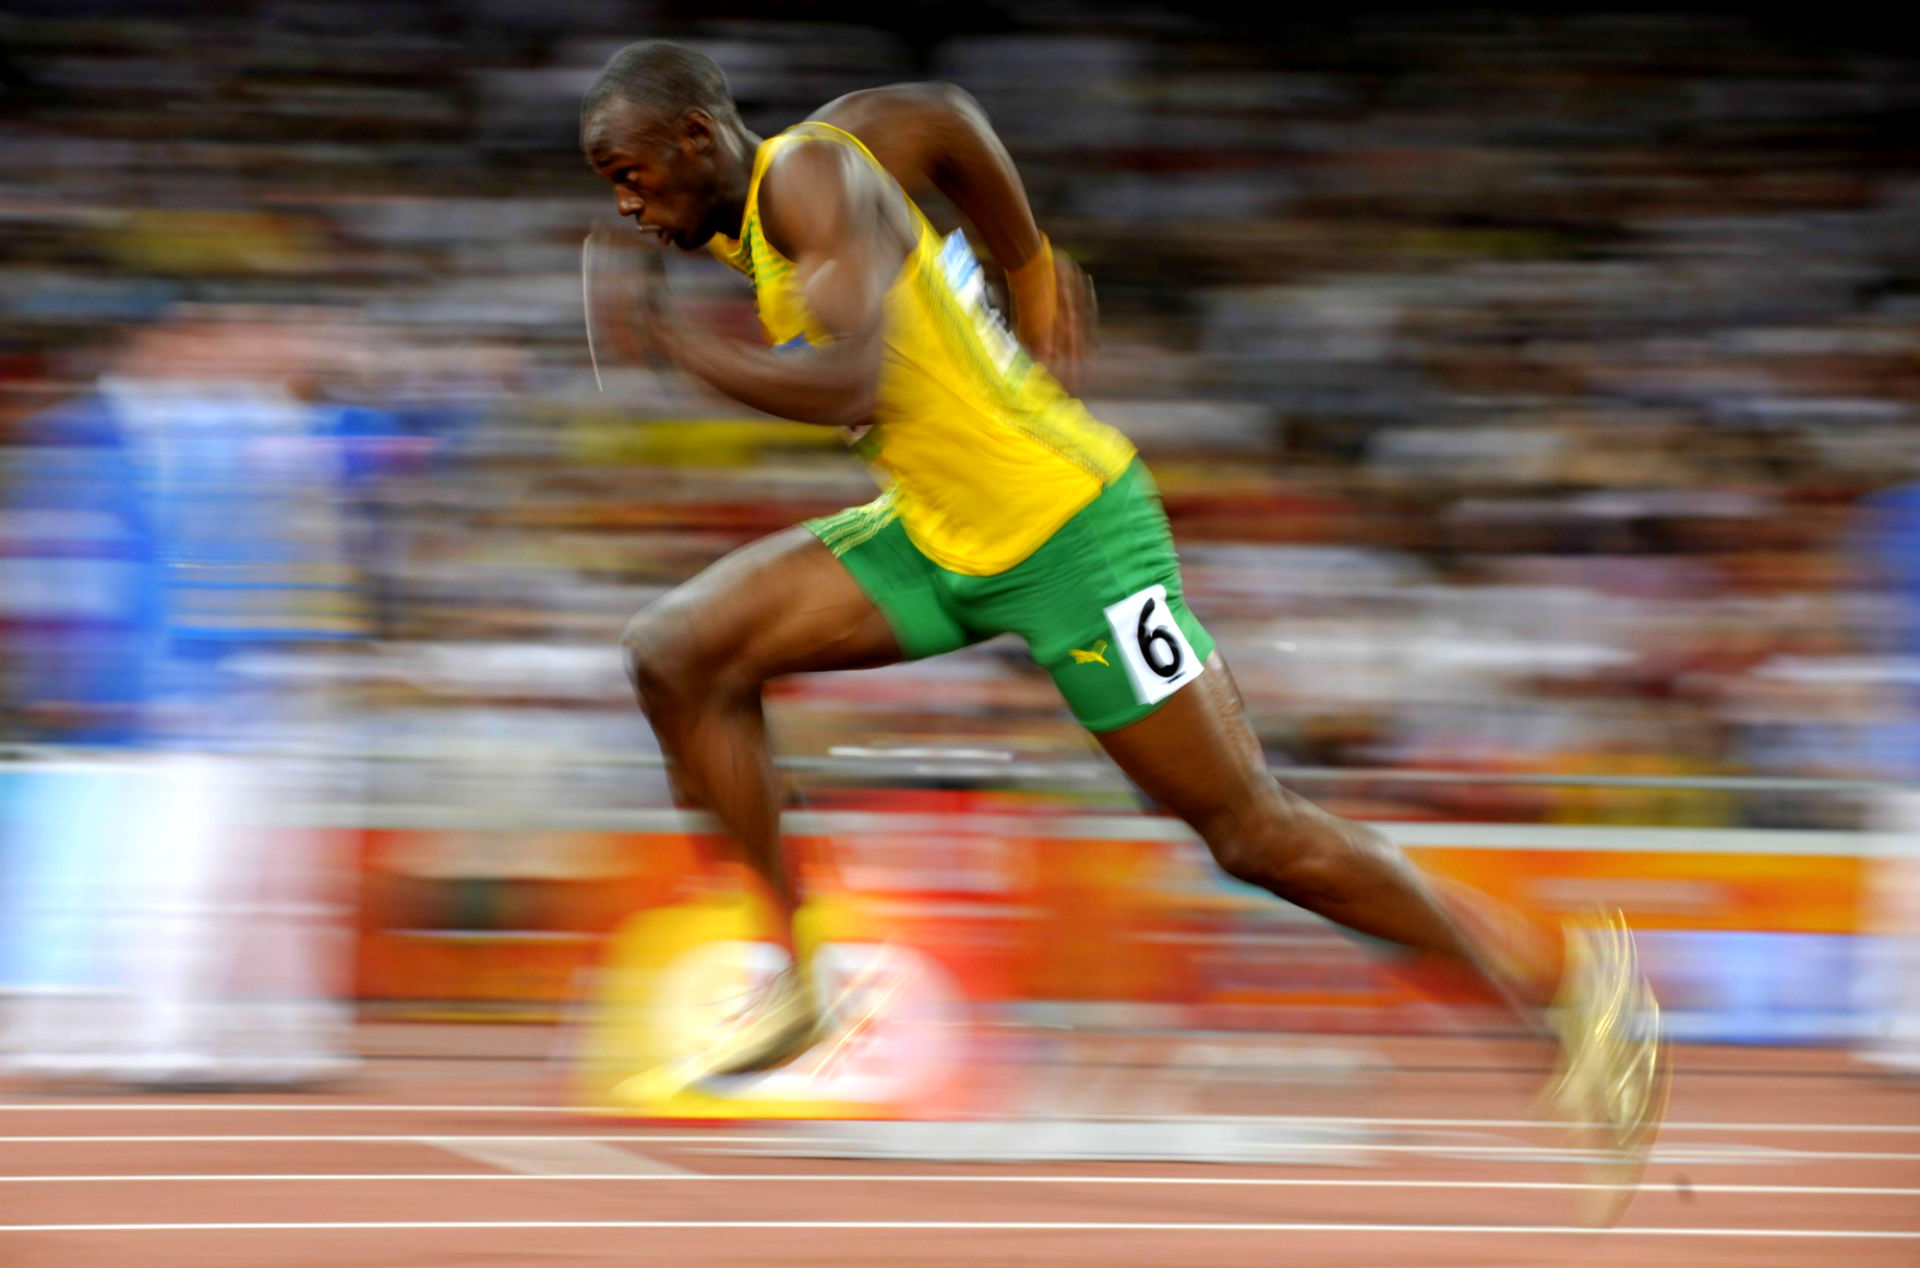
\includegraphics[scale=0.053]{bolt.png}\\
       \end{block}
  $\Downarrow$ (Validation)
      \begin{block}{Mathematical Model}
       \center
       $\frac{d^2x(t)}{dt^2} = \frac{F}{M}$\\
      \end{block}
  $\Downarrow$ (Verification)
  \begin{block}{Numerical Representation}
   \center
   $\frac{d^2x}{dt^2} = f''(t) = \frac{f(t+h) - 2 f(t) + f(t-h)}{h^2} + \textcolor{red}{?}$
   \end{block}
 \end{center}
\end{frame}
%

\begin{frame}
 %\frametitle{Verification, Validation and Uncertainty Quantification}
 \frametitle{What is Validation?}

 \begin{block}{The Scientific Method}
  \begin{itemize}
  \item Predictive Simulation: systemic treatment of model and data uncertainties and their
    propagation through a computational model to produce predictions
    of quantities of interest with quantified uncertainty
  \item Goal: use scientifically-based predictions of physical reality to make informed decisions
    \begin{itemize}
    \item Often, mathematical constructs (e.g., equations)
    \end{itemize}
    Falsifiable: if predictions are ``wrong'' model is not valid
  \end{itemize}
 \end{block}

\end{frame}
%
%
%
\begin{frame}
 %\frametitle{Verification, Validation and Uncertainty Quantification}
 \frametitle{What is Validation?}

 \begin{block}{Some Tough Questions in Validation}
  \begin{itemize}
  \item Predictive Simulation: systemic treatment of model and data uncertainties and their
    propagation through a computational model to produce predictions
    of quantities of interest with quantified uncertainty
  \item Goal: use scientifically-based predictions of physical reality to make informed decisions
    \begin{itemize}
    \item Often, mathematical constructs (e.g., equations)
    \end{itemize}
    Falsifiable: if predictions are ``wrong'' model is not valid
  \end{itemize}
 \end{block}

\end{frame}
%
%
%
%===============================================================================
% slide 1
\begin{frame}
\frametitle{How close is close enough?}

\begin{block}{It depends:}
  \begin{itemize}
   \item on your quantity of interest
   \item on where you are predicting (extrapolation?)
   \item on how risky the action is
   \item how ``physics-based'' is the model
  \end{itemize}
\end{block}

\centering
Any validation study must involve uncertainty quantification

\end{frame}

%************************************************
% New section
%************************************************
\section{A clean UQ example}

%===============================================================================
% slide 1
\begin{frame}
\frametitle{A clean UQ example}

 \begin{block}{Direct Numerical Simulation (DNS) as a Computational Laboratory}
  \begin{itemize}
   \item Resolve all relevant physical scales (large and small)
   \item DNS data is widely used by the turbulence community
   \item Errors and uncertainties are seldom quantified 
 \end{itemize}

 \end{block}

 \begin{block}{Typical practice}
  \begin{itemize}
   % todo make this better
  \item Mesh resolution and simulation time guided by previous experience
  \item Results evaluated by expert practitioners looking for:
    \begin{itemize}
    \item Non-stationary behavior, insufficient sampling
    \item Insufficient resolution
    \end{itemize}
  \item Almost entirely qualitative
  \end{itemize}
\end{block}

\end{frame}

\section{Methodology}

%==============================================================================
\begin{frame}
\frametitle{Error Decomposition}

\vfill

\begin{equation*}
  \langle q_h \rangle_{N} = \langle q \rangle + e_h + \epsilon_{h,N}
\end{equation*}

\vfill

\begin{description}
\item[$q_h$] Instantaneous value of QoI at resolution $h$
\item[$\langle q_h \rangle_{N}$] Computed mean at resolution $h$ with sampling duration $N$
\item[$\langle q \rangle$] ``True'' mean value of QoI ($h \rarrow 0$, $N \rarrow \infty$)
\item[$e_h$] Discretization error at resolution $h$ ($N \rarrow \infty$)
\item[$\epsilon_{h,N}$] Sampling error at resolution $h$ for sampling duration $N$
\end{description}

\vfill

Require methods to estimate both $e_h$ and $\epsilon_{h,N}$

\vfill

\end{frame}

\subsection{Statistical error estimation: Autoregressive modeling}


%==============================================================================
% slide 2
\begin{frame}
\frametitle{Estimating Statistical Error, $\epsilon_{h,N}$}

 \begin{block}{CLT, Regained}
  \begin{itemize}
  \item How to characterize the statistical error?
	\begin{itemize}	   
	 %\item $\epsilon_{h,N} \rightarrow $ Gaussian
	 \item $\epsilon_{h,N} \overset{d}{\rarrow} \mcal{N}(0, \sigma^2/N)$
	       in limit of large (independent) sample size
	 \item Calculate ``decorrelation time'': $N_0$
	 \item ``effective sample size'': $N_\text{effective} = N / N_0$
	 \item Regain CLT convergence:
	       $\frac{1}{\sqrt{N_\text{effective}}}$ 
	\end{itemize}
  \end{itemize}
 \end{block}

 \begin{block}{Computing the Autocorrelation}
   \begin{itemize}	
    \item Computing $N_0$ requires the
	  autocorrelation function, $\rho$
	  \begin{itemize}
	   \item Direct calculations of $\rho$ from $O(100)$ samples is noisy
	  \end{itemize}
    \item Instead, $\rho$ estimated using maximum entropy
	  autoregressive model fitting as in Trenberth (1984)
   \end{itemize}
 \end{block}

\end{frame}


\subsection{Discretization error estimation: Bayesian Richardson Extrapolation}
%===============================================================================
% \begin{frame}
% \frametitle{Bayesian Richardson Extrapolation}

% By Bayes' theorem:
% %
% \begin{equation*}
% \underbrace{\pi \left(\avg{q}, C, p | \avg{q_h}_N\right)}_{\mathrm{Posterior}} 
% \propto 
% \underbrace{\pi \left( \avg{q}, C, p \right)}_{\mathrm{Prior}} \, 
% \underbrace{L \left(\avg{q}, C, p; \avg{q_h}_N \right)}_{\mathrm{Likelihood}}
% \end{equation*}
% %
% where
% %
% \begin{itemize}
% \item Prior depends on knowledge of the problem; we use ``broad'' priors
% \item Likelihood formed from statistical error model:
% \begin{equation*} 
% L \left(\avg{q}, C, p; \avg{q_h}_N \right) = \prod_{i=1}^3 \Phi \left( \avg{q_{h_i}}_N - \avg{q} - C h_i^p; \frac{\hat{\sigma}_N^2 T_0}{N} \right).
% \end{equation*}
% where
% \begin{equation*}
% \Phi(x;s^2) = \frac{1}{\sqrt{2 \pi s^2}} \exp \left( -\,\frac{1}{2} \frac{x^2}{s^2} \right)
% \end{equation*}
% \item Note that the Gaussian assumption here is based on the extended
%   CLT given before
% \end{itemize}

% \end{frame}

\begin{frame}
\frametitle{Estimating Discretization Error, $e_h$}

\begin{block}{Deterministic (Standard Richardson Extrapolation)}
\begin{itemize}
\item Assume: $q_h = q + C h^p$
\item Given $q_h$ for 3 distinct $h$, solve for $q$, $C$, and $p$
\item Breaks down when $q_h$ contaminated by sampling error
\end{itemize}
\end{block}

\begin{block}{Stochastic (Bayesian Richardson Extrapolation)}
\begin{itemize}
\item Recall our model: $\langle q_h \rangle_{N} = \langle q \rangle + e_h + \epsilon_{h,N}$
%$\avg{q_h}_N = \avg{q} + e_h + \epsilon_{h,N}$
\item Assume: $e_h = C h^p$
  \begin{itemize}
  \item Other models may be appropriate depending on the discretization
  \end{itemize}
 \item \emph{Infer} $\langle q \rangle$, $C$, and $p$ under uncertainty imposed by
      $\epsilon_{h,N}$
 \item We choose a Bayesian approach to the inverse problem
 \item Prior depends on knowledge of the problem; we use ``broad'' priors
\end{itemize}
\end{block}

\end{frame}

\section{Results}

\subsection{An Aside}

%===============================================================================
%     MCMC -- what is it?
%===============================================================================
\begin{frame}
  \frametitle{MCMC}

  \begin{block}{What is it?}
    \begin{itemize}
    \item \textcolor{black}{M}CMC = \textcolor{black}{Markov} Chain Monte-Carlo
    \item \textcolor{black}{Markov = Each step only depends on previous}
    \item Chain = A series of steps
    \item Monte-Carlo = Stochastic (i.e. random numbers)
    \end{itemize}
    Essentially, a method to generate random steps \textcolor{black}{correlated with the previous step}

  \end{block}
\end{frame}

%===============================================================================
%     Picture Example: reject
%===============================================================================
\begin{frame}
\frametitle{Enter Metropolis-Hastings}
\begin{block}{Intuitive Picture: Sampling a Gaussian Distribution}
\centering
  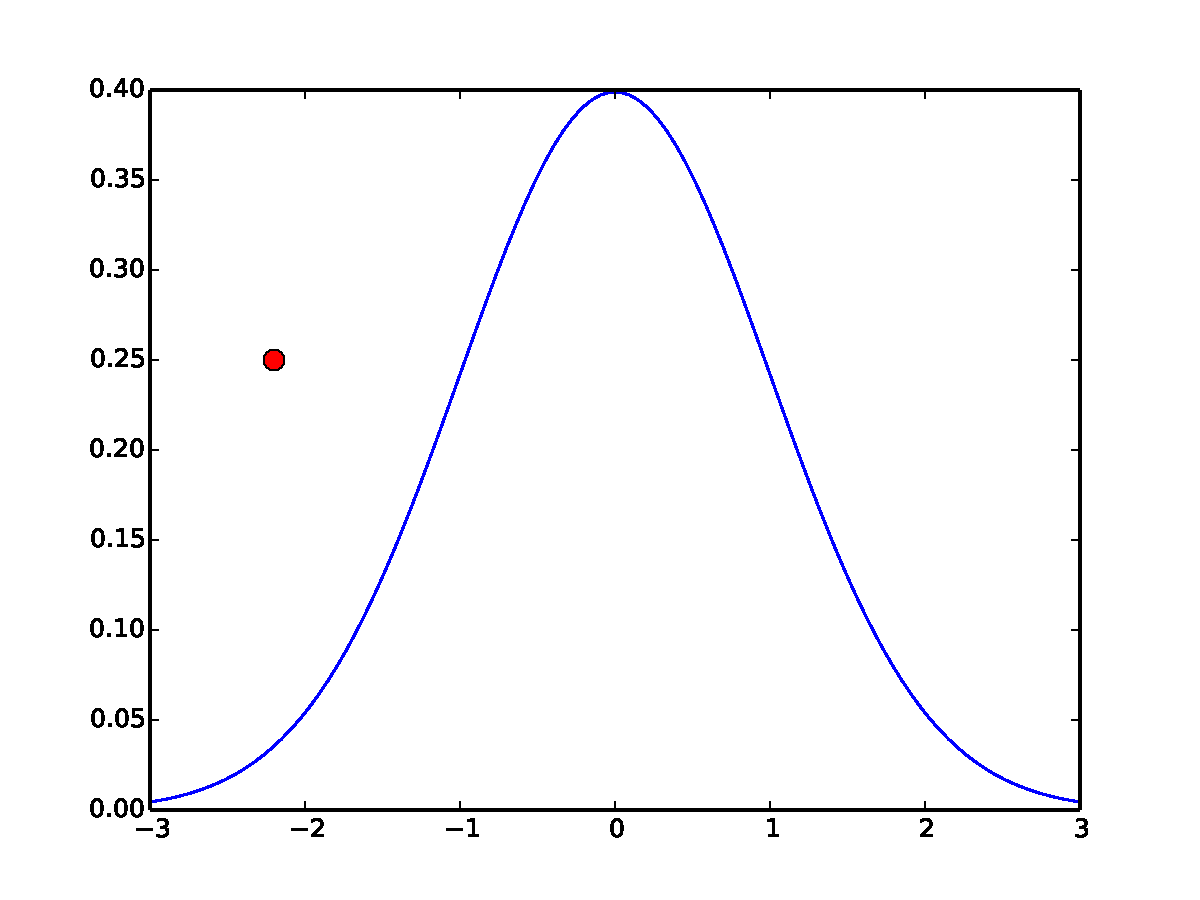
\includegraphics[width=3.5in]{figs/norm.pdf}
\end{block}

\end{frame}

%===============================================================================
%     picture sample one: accept
%===============================================================================
\begin{frame}
\frametitle{Enter Metropolis-Hastings}

\begin{block}{Intuitive Picture: Sampling a Gaussian Distribution}
\centering
  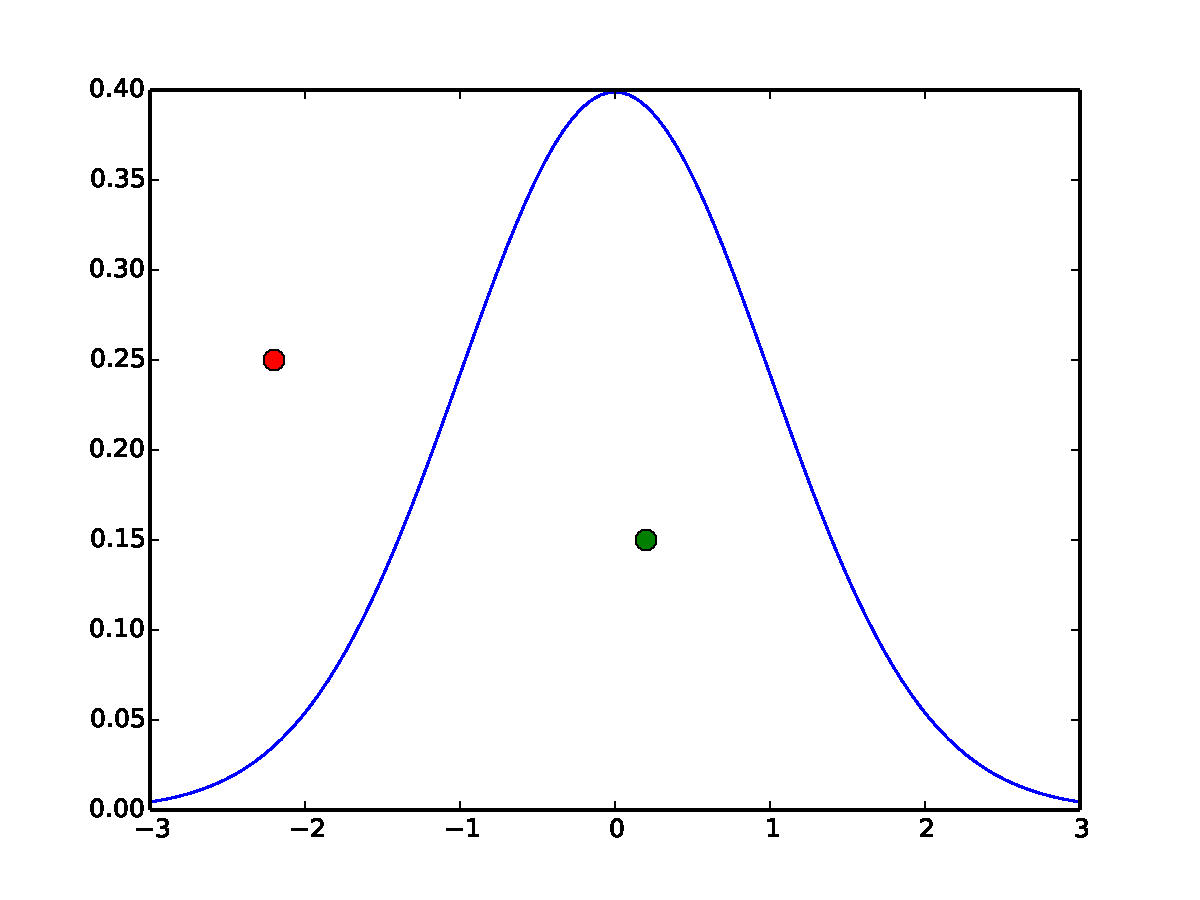
\includegraphics[width=3.5in]{figs/norm-acc.pdf}
\end{block}

\end{frame}

%===============================================================================
%     picture sample one: correlated
%===============================================================================
\begin{frame}
\frametitle{Enter Metropolis-Hastings}

\begin{block}{Intuitive Picture: Sampling a Gaussian Distribution}
\centering
  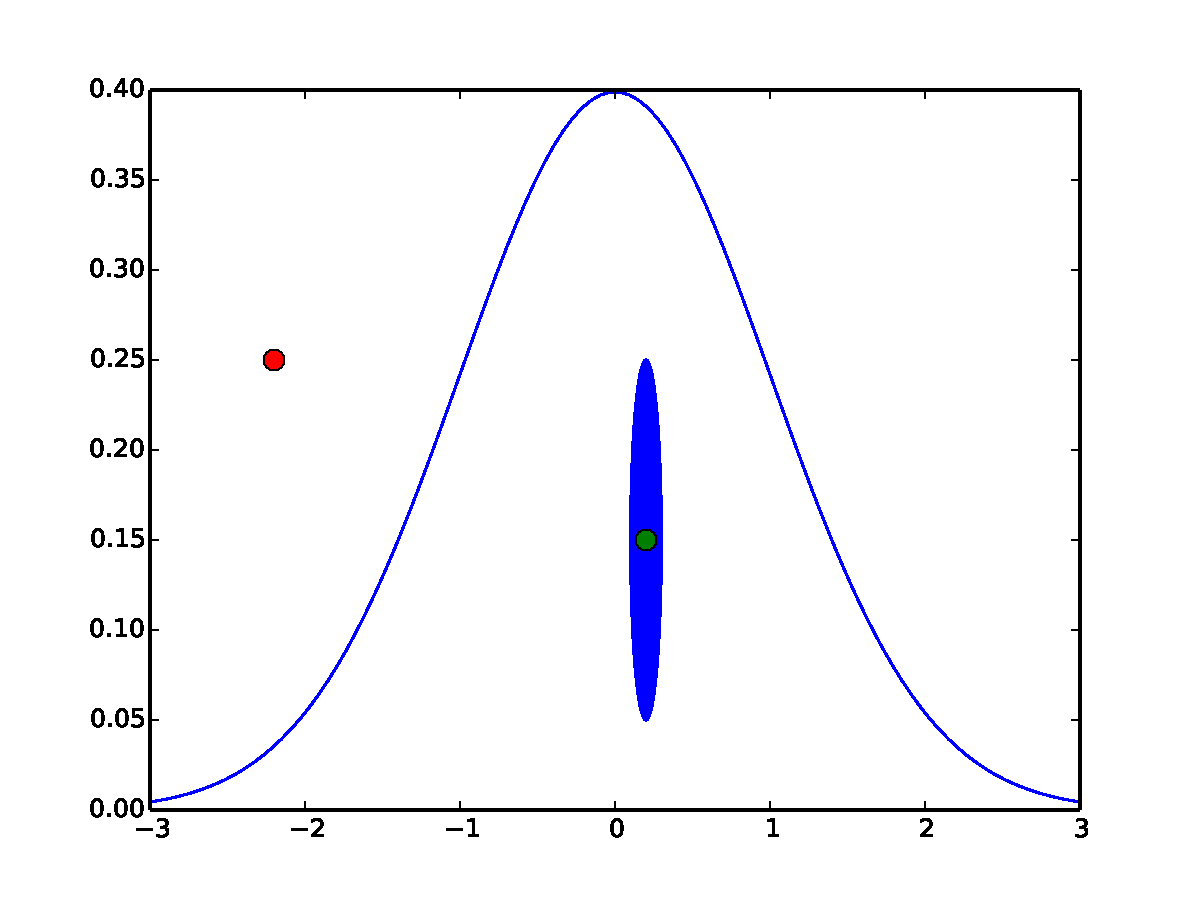
\includegraphics[width=3.5in]{figs/norm-corr.pdf}
\end{block}

\end{frame}

%===============================================================================
%     So... what is metropolis-hastings?
%===============================================================================
\begin{frame}
\frametitle{Enter Metropolis-Hastings}

\begin{block}{What is it?}
  \begin{itemize}
  \item Metropolis-Hastings is an MCMC method for generating these samples. 
  \end{itemize}
\end{block}

\begin{block}{Algorithm}
  \begin{itemize}
  \item Start at current step ($\phi_1$)
  \item Draw proposal: $q(\tilde \phi_2 | \phi_1) = N(\tilde \phi_2 | \phi_1, \nu^2)$
  \item Draw from uniform: $u \sim U(0,1)$
  \item if: $u < \frac{\pi_n(\tilde \phi_2)}{\pi_n(\phi_1)}$ ($\pi_n$ is bayesian posterior, etc.)
    \begin{itemize}
    \item $\phi_2 = \tilde \phi_2$
    \end{itemize}
  \item else: $\phi_2 = \phi_1$
  \end{itemize}
\end{block}

\textcolor{red}{Question: How do we choose $\nu$?}

\end{frame}
%
%
%
%===============================================================================
%     Picture Example: reject
%===============================================================================
\begin{frame}
\frametitle{Metropolis-Hastings Sampling: Convergence}

\begin{block}{Sampling a Gamma Distribution}
  \begin{columns}
  \column{0.35\textwidth}
    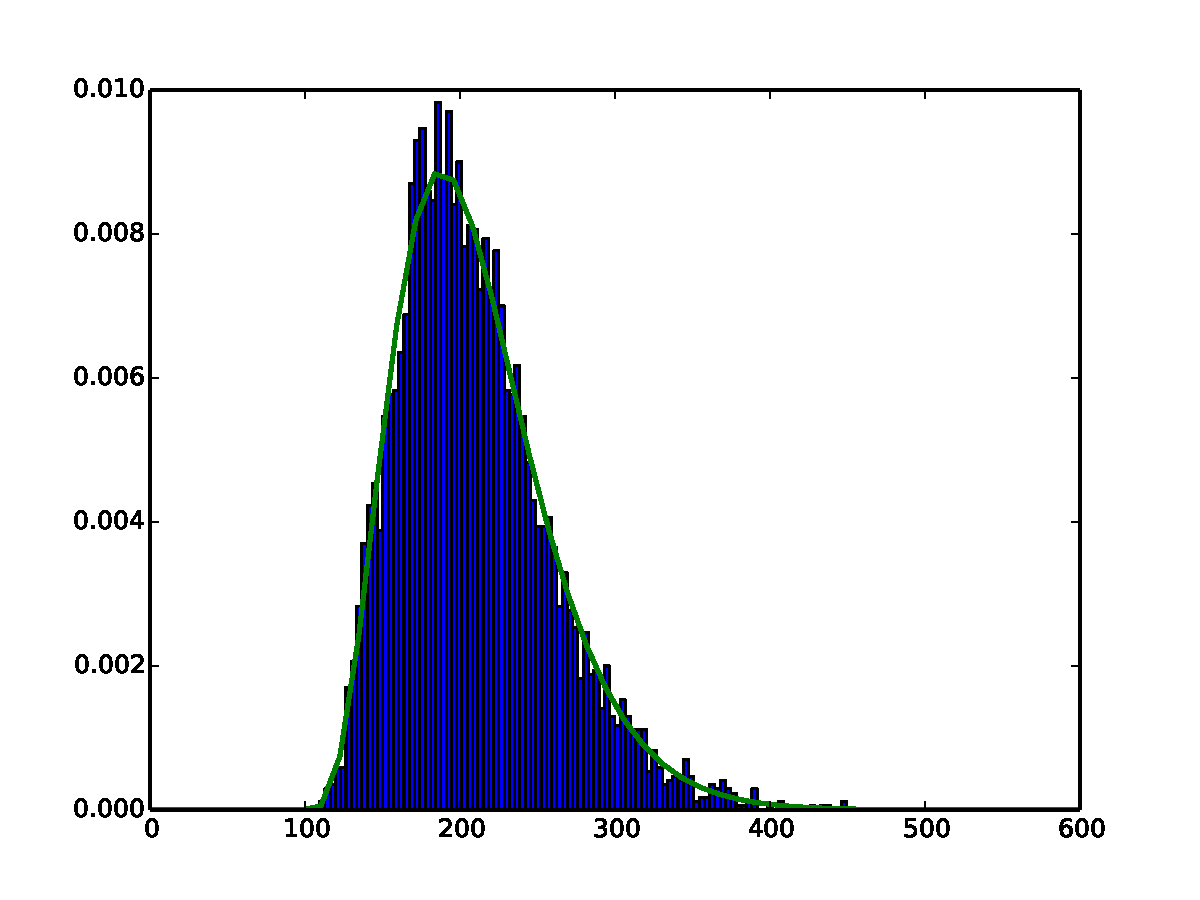
\includegraphics[width=2.5in]{figs/gamma.pdf}

  \column{0.5\textwidth}
  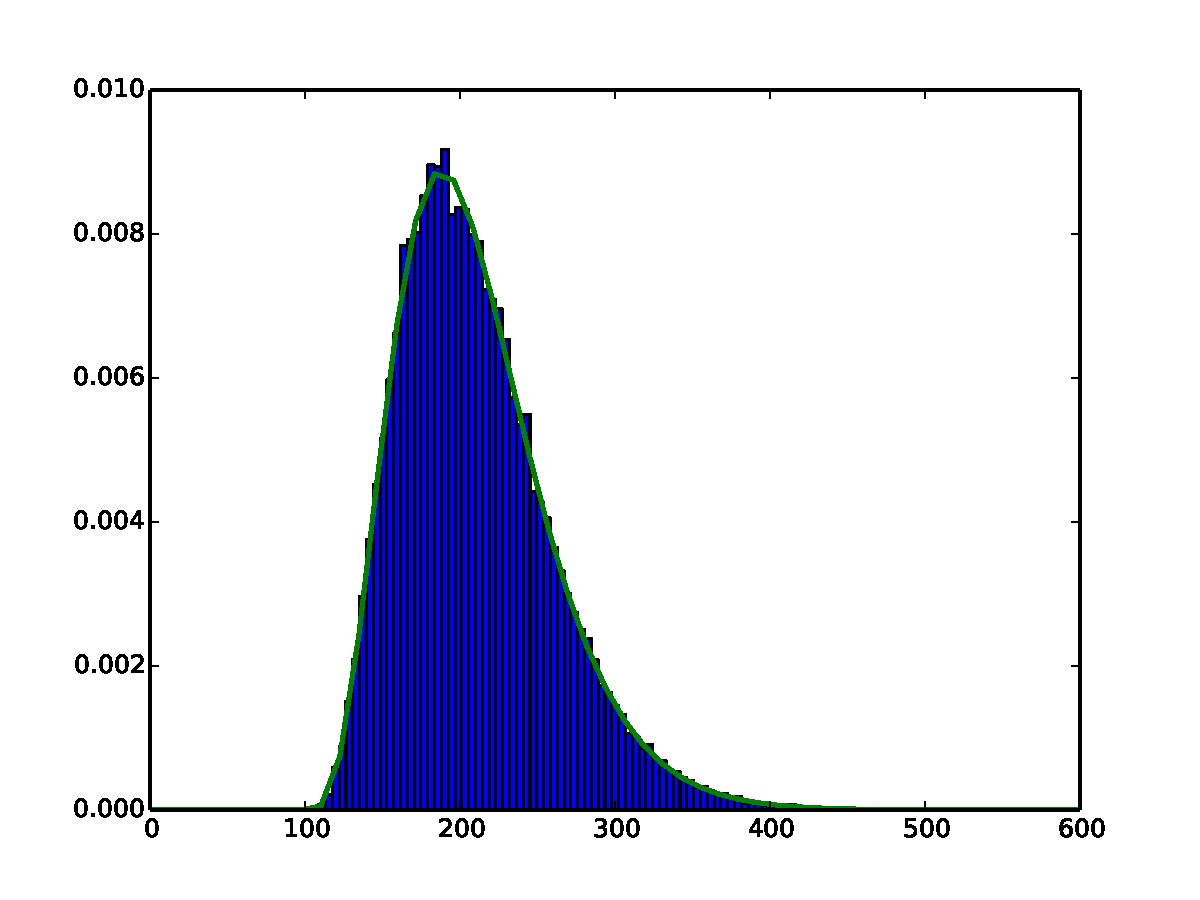
\includegraphics[width=2.5in]{figs/gamma_50k.pdf}
  \end{columns}
\end{block}

\end{frame}


%===============================================================================
%     OpenMP intro
%===============================================================================
\begin{frame}
\frametitle{Burn-in}

\begin{block}{MCMC Chain}
\begin{itemize}
\item That initial guess can lead to many rejections
\end{itemize}		  
\centering
  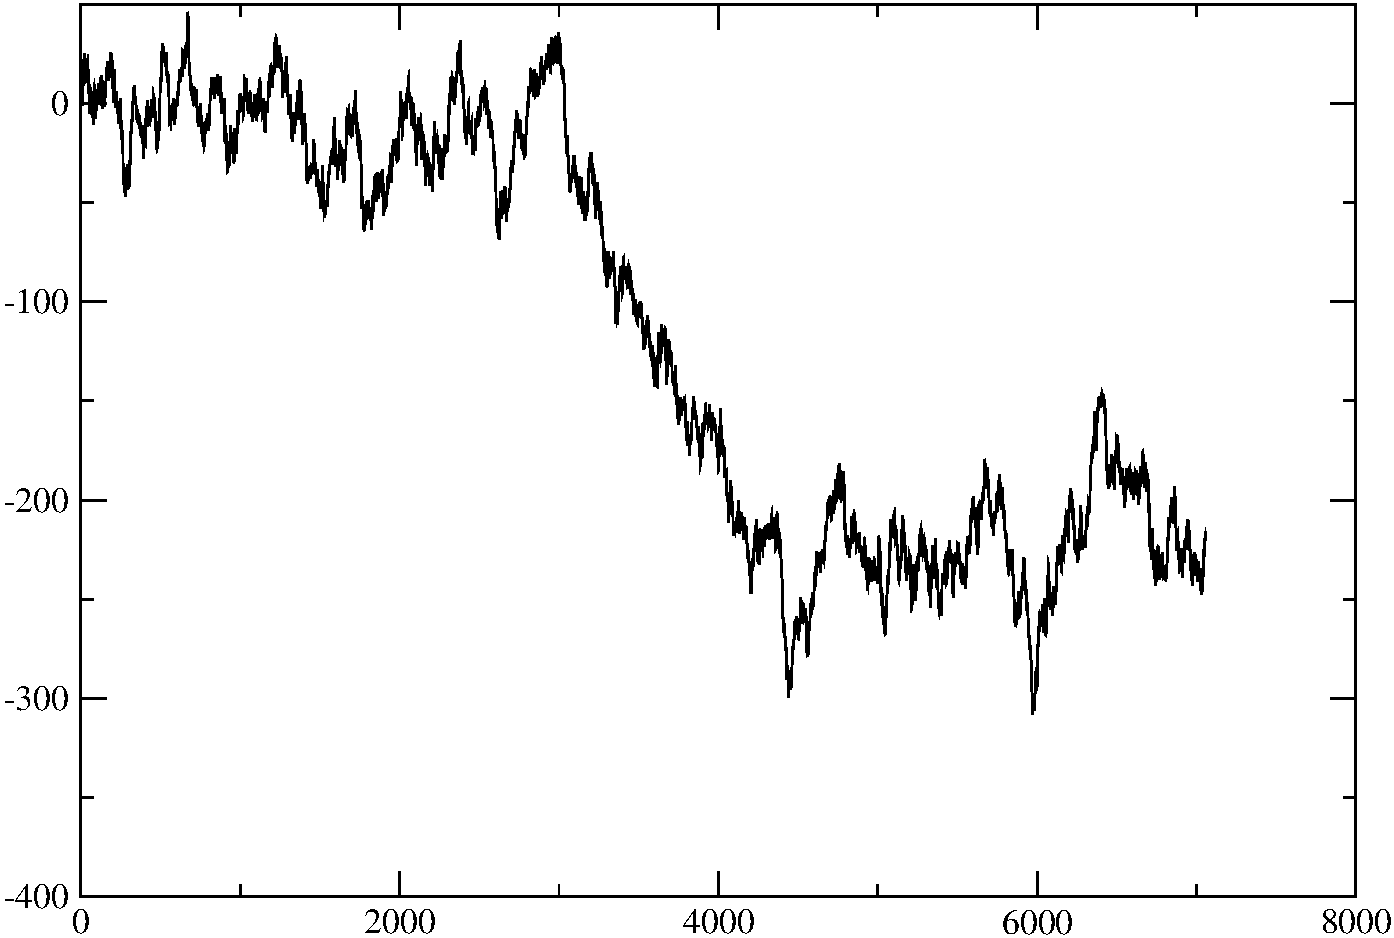
\includegraphics[width=3.5in]{figs/example.pdf}
\end{block}

\end{frame}

%
\subsection{Lorenz equations}
%===============================================================================
\begin{frame}
\frametitle{Verification of Methodology: Lorenz Equations}
%
\begin{columns}[]
  \begin{column}{0.33\linewidth}
    \begin{center}
      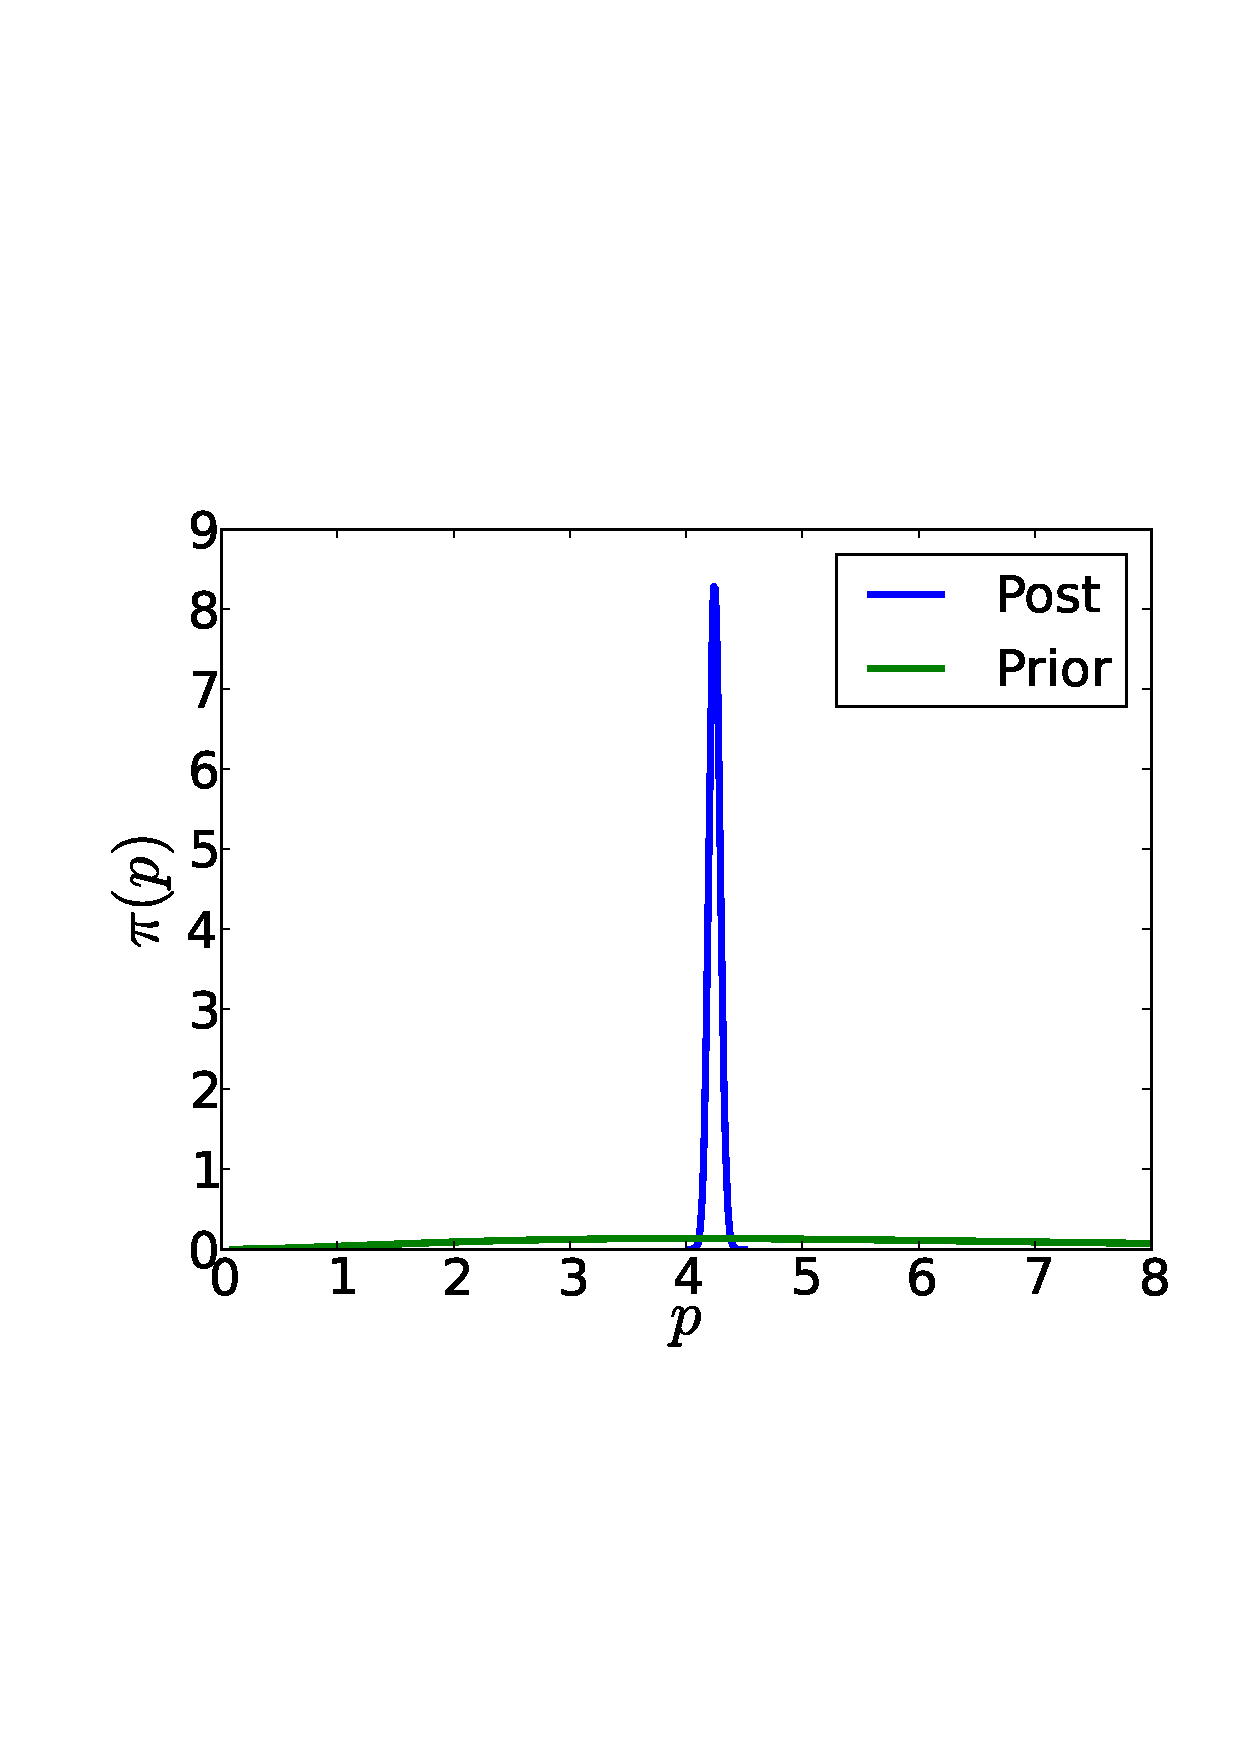
\includegraphics[width=0.99\linewidth]{p_post_sharp.pdf}
    \end{center}
  \end{column}
  %
  \begin{column}{0.33\linewidth}
    \begin{center}
      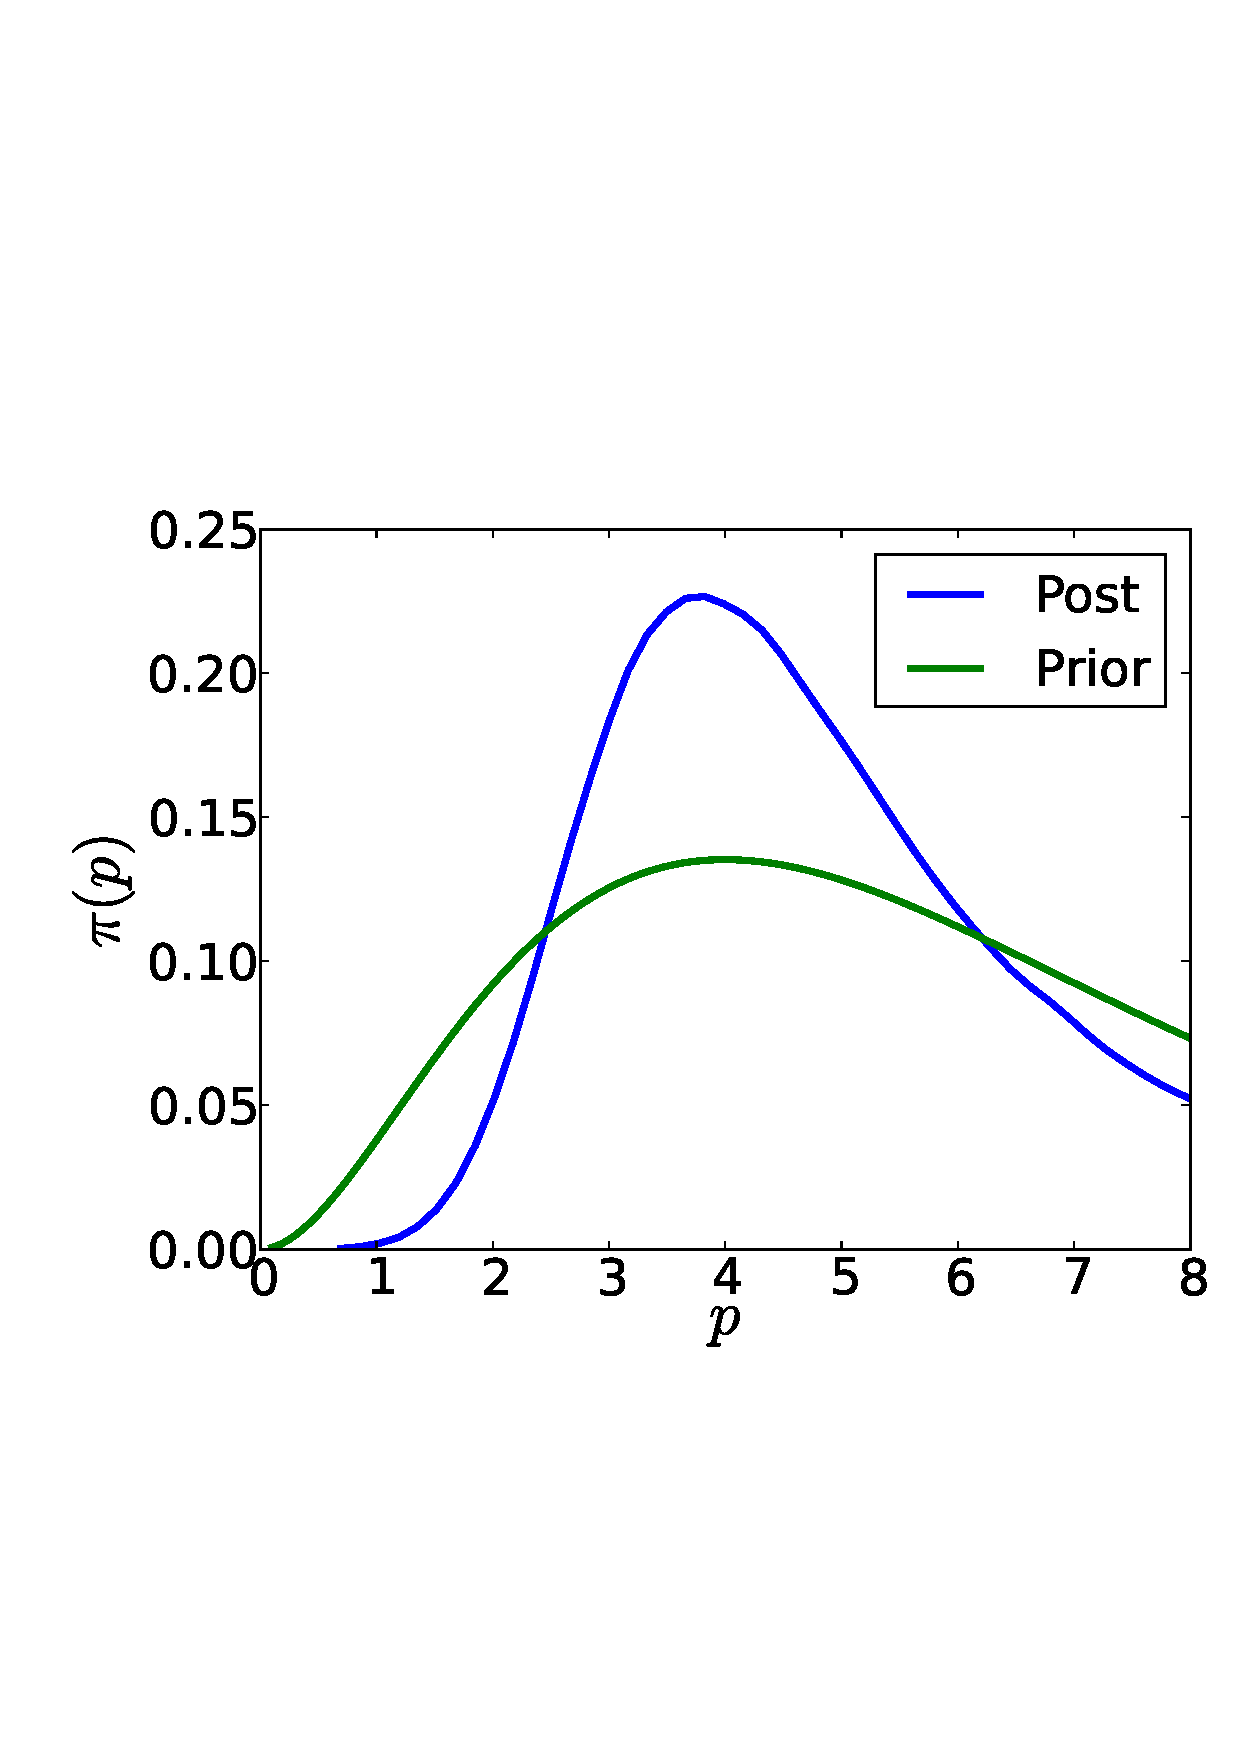
\includegraphics[width=0.99\linewidth]{p_post_mid.pdf}
    \end{center}
  \end{column}
  %
  \begin{column}{0.33\linewidth}
    \begin{center}
      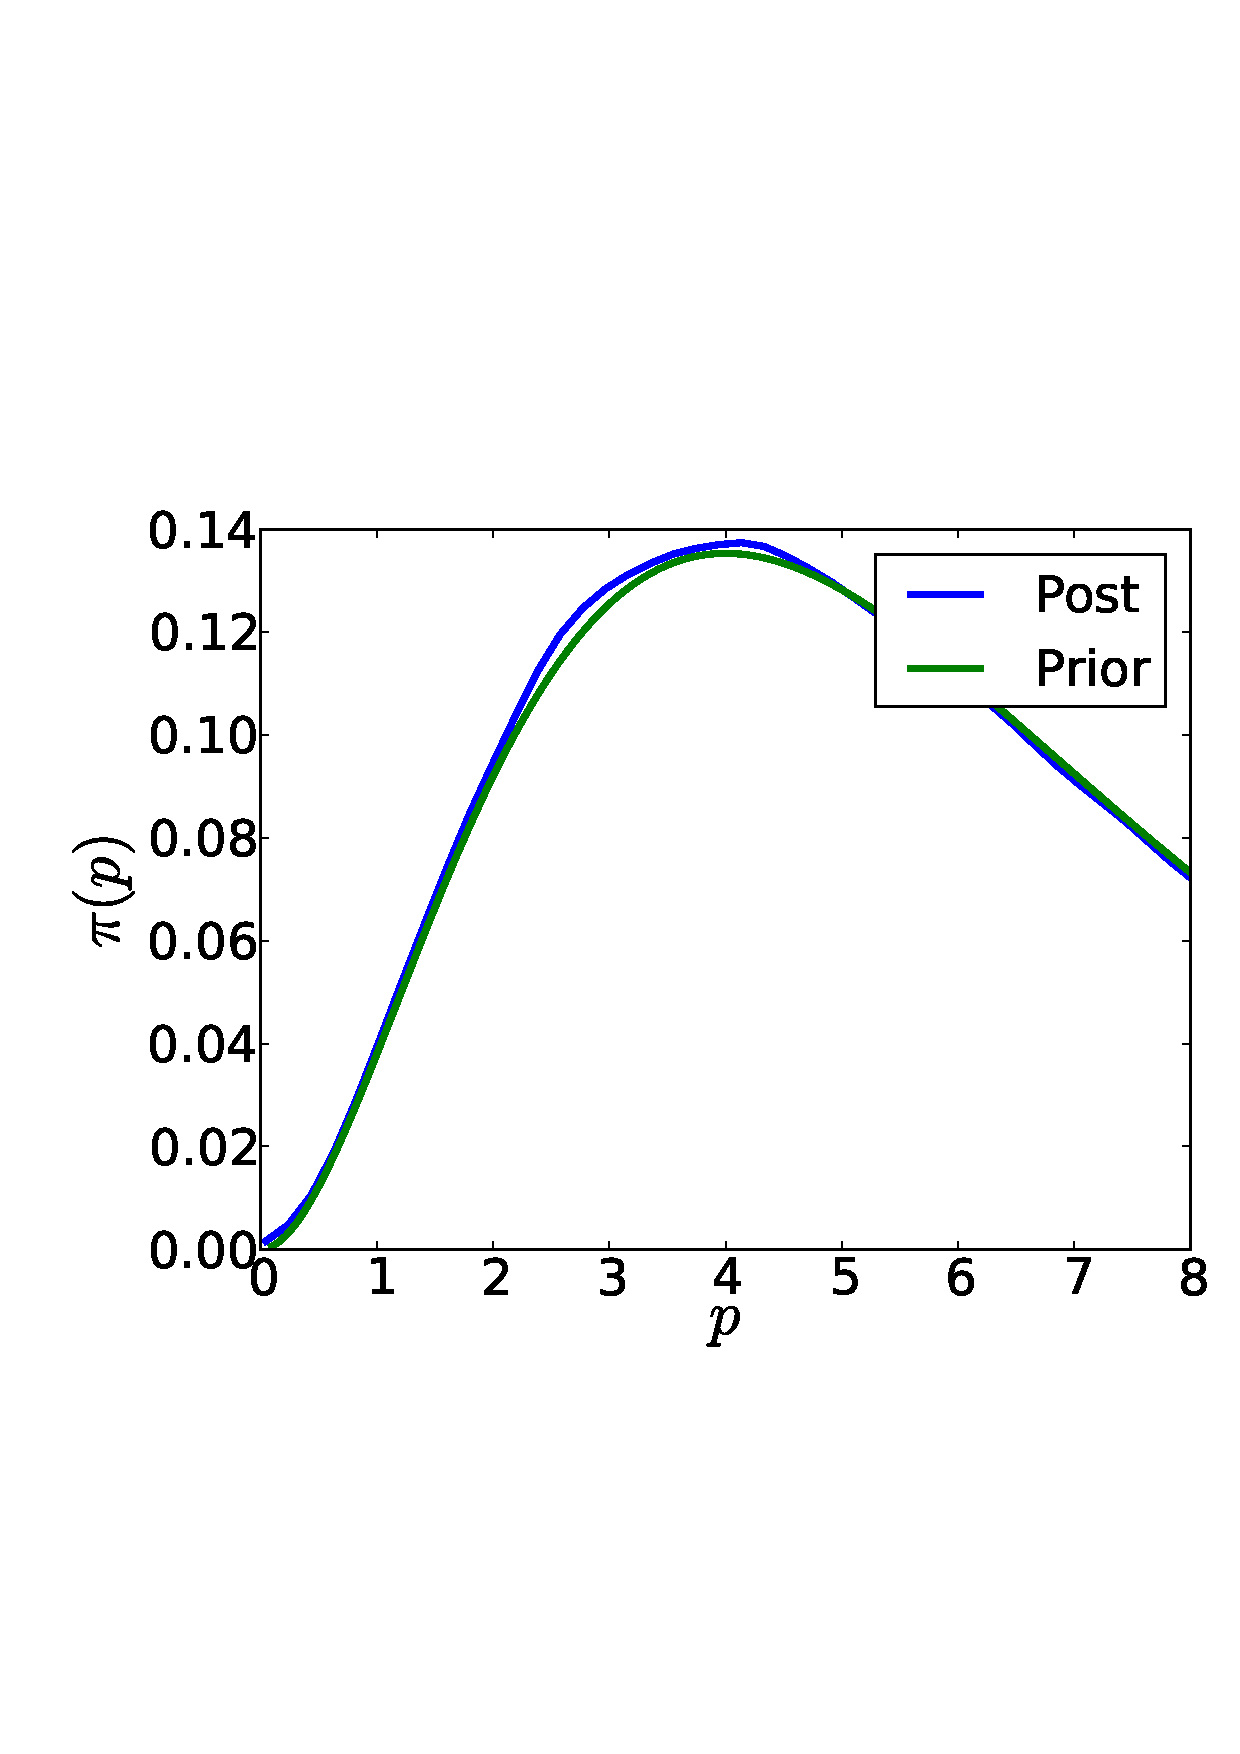
\includegraphics[width=0.99\linewidth]{p_post_noisy.pdf}
    \end{center}
  \end{column}
\end{columns}

\setlength{\unitlength}{\linewidth}
\linethickness{1.5pt}
\begin{picture}(0.8, 0.05)(-0.1,0)
\put(0,0.03){\vector(1,0){0.8}}
\put(0,0){\makebox(0.8,0){Increasing statistical uncertainty}}
\end{picture}

\vspace{0.1in}
\begin{block}{}
\begin{itemize}
\item Using RK4 $\Rarrow \,\, p=4$
\item Only recover true $p$ with small statistical uncertainty
\item With large statistical uncertainty, posterior same as prior
\end{itemize}
\end{block}

\end{frame}

\subsection{$Re_\tau = 180$ Channel Flow}
%===============================================================================
\begin{frame}
 \begin{block}{Numerical Methods}
  \begin{itemize}
   \item Fourier--Galerkin in streamwise (x) and spanwise (z)
   \item B-spline collocation in wall-normal (8th order B-splines)
   \item SMR91 hybrid implicit/explicit time scheme\footnotemark[4]
      (Mixed $2^\text{nd}$ and $3^\text{rd}$ order.)
  \end{itemize}
 \end{block}

% \begin{block}{Case Details $\text{Re}_{\text{bulk}} = U \delta / \nu = 2925$}
% \begin{itemize}
% \item Box size\footnotemark[5]: $L_x/\delta = 4 \pi$, $L_z/\delta = 2 \pi$
% \item Nominal mesh designed according to standard heuristics
%   \begin{itemize}
%   \item Points ($x \times y \times z$): $192 \times 128 \times 192$
%   \item Resolution: $\Delta x^+ \approx 11.8$, $\Delta z^+ \approx 5.9$, $\Delta y^+_{\text{wall}} \approx 0.16$, $\Delta y^+_{CL} \approx 4.4$
%   \end{itemize}
% \item Nominal $\Delta t (U / \delta) = 0.01$; Always $<$ CFL limit
% \item Additional cases via uniform coarsening/refinement: Coarsest ($h=2$); Coarse ($h=\sqrt{2}$); Nominal ($h=1$); Finest ($h=1/2$)
% \end{itemize}
% \end{block}
% \footnotetext[4]{\tiny{Spalart, Moser, and Rogers, \emph{Journal of Computational Physics}, 1991.}}
% \footnotetext[5]{\tiny{Kim, Moin, and Moser, \emph{Journal of Fluid Mechanics}, 1987.}}
% 

\footnotesize
\begin{table}
\begin{tabular}{|l|rrr|rccc|rl|}
\hline
Name & $N_x$ & $N_z$ & $N_y$ & $\Delta x^+$ & $\Delta
 z^+$ & $\Delta
 y^+_{\rm wall}$ & $\Delta y^+_{\rm CL}$ & $T U_b / L_x$ & $\Delta t U_b
 / \delta$ \\
\hline
Coarsest  &   96 &  96 &  64 & 24.3 & 12.2 & 0.44 &
				     9.14 & 2651.0 &0.02\\
Coarse    &  136 & 136 &  90 & 17.2 &  8.6 & 0.26 &
				     6.46 &  273.5 &0.01414\\
Nominal   &  192 & 192 & 128 & 12.2 &  6.1 & 0.16 &
				     4.53 & 2145.3 &0.01\\
Finest    &  384 & 384 & 256 &  6.1 & 3.0 & 0.07 &
				     2.26 &  709.3 &0.005\\
\hline
\end{tabular}
 \label{tbl:channel_runs}
\end{table}

 \normalsize
 \begin{block}{Case Details}
  \begin{itemize}
   \item $\text{Re}_{\tau} \approx 180$, $\text{Re}_{\text{bulk}} = U \delta / \nu = 2925$
   \item Box size\footnotemark[5]: $L_x/\delta = 4 \pi$, $L_z/\delta = 2
	 \pi$
   \item $\Delta t $ always $<$ CFL limit
  \end{itemize}
 \end{block}
 \footnotetext[4]{\tiny{Spalart, Moser, and Rogers, \emph{Journal of Computational Physics}, 1991.}}
 \footnotetext[5]{\tiny{Kim, Moin, and Moser, \emph{Journal of Fluid Mechanics}, 1987.}}

\end{frame}

%===============================================================================
\begin{frame}
\frametitle{Results of the Inverse Problem for $U_\text{CL}$}

    \begin{center}
     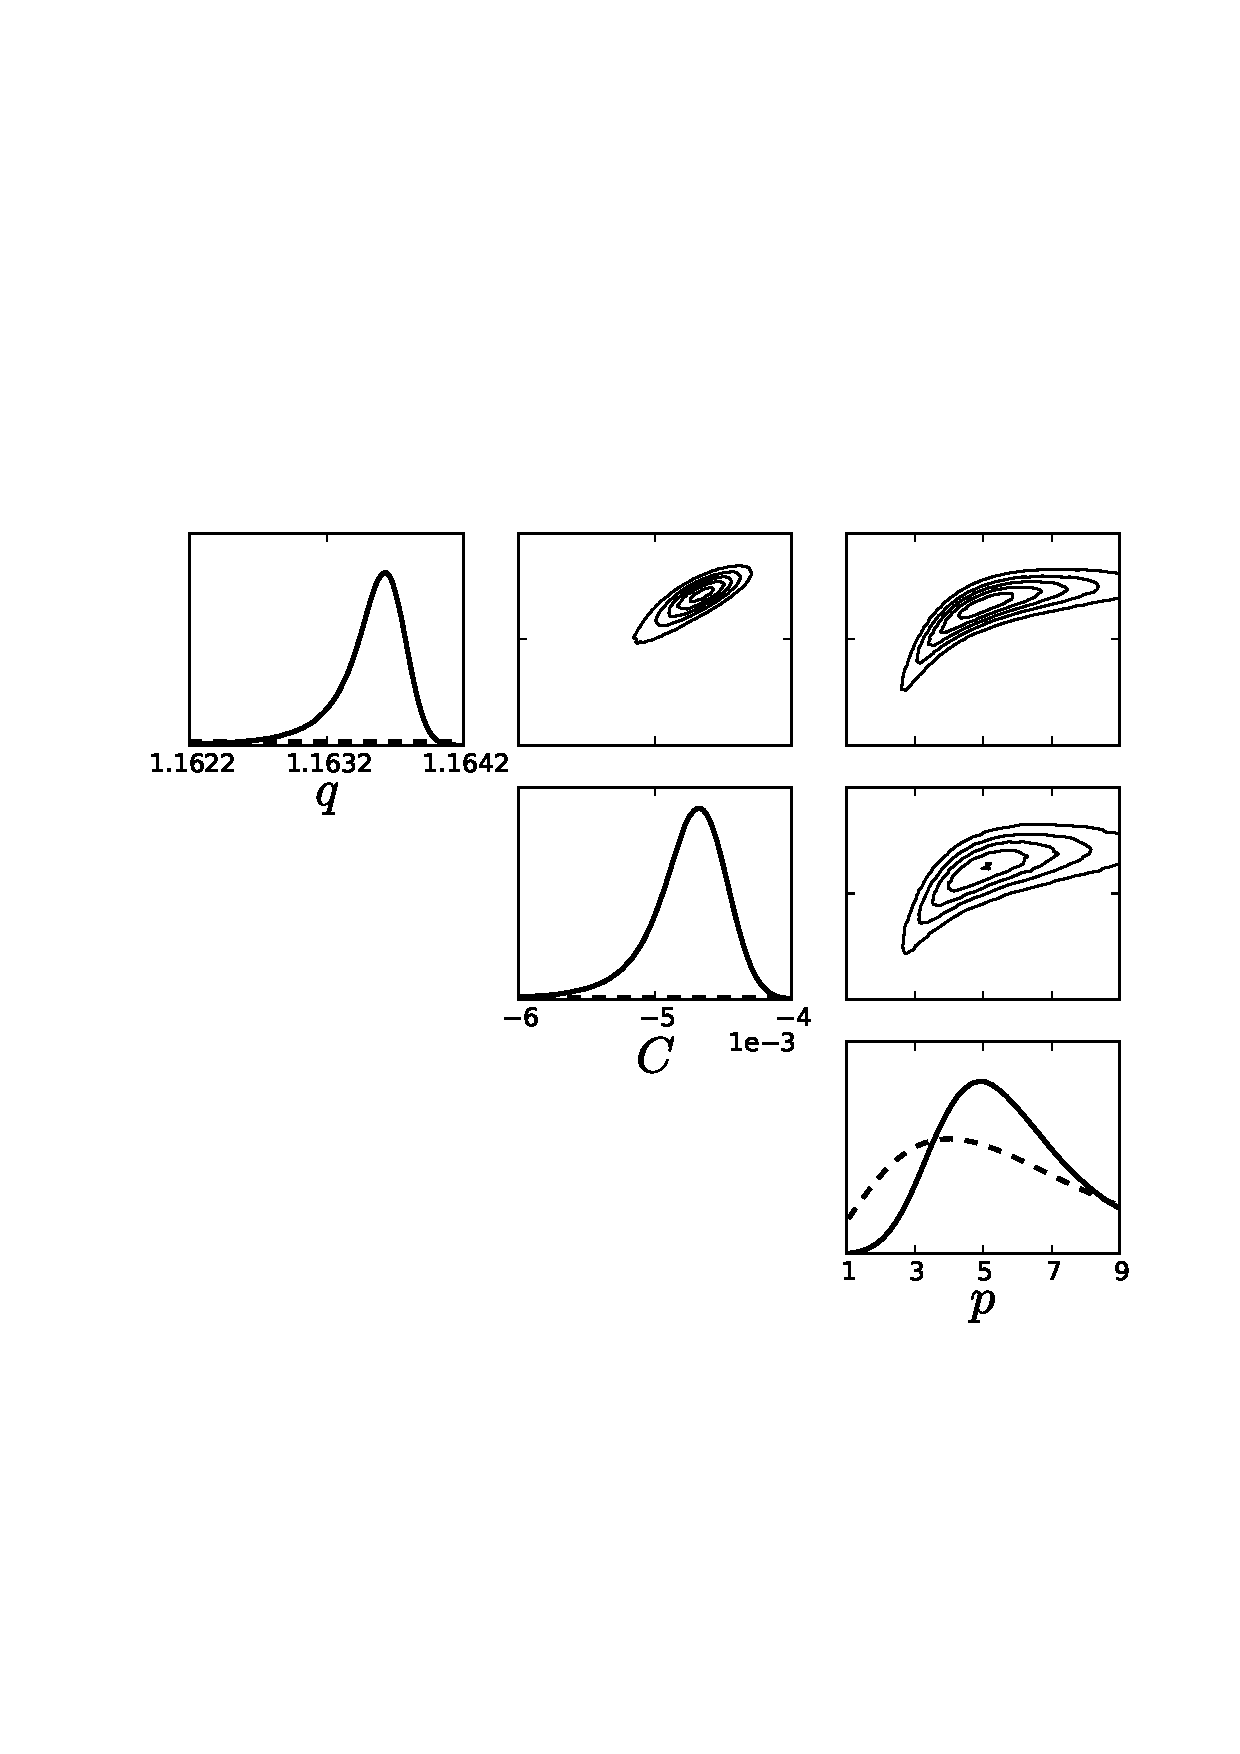
\includegraphics[width=0.8\linewidth]{cl_chp_joint_post.pdf}
    \end{center}

\end{frame}

%===============================================================================
\begin{frame}
\frametitle{Results of the Calibration for the Centerline Velocity}

\begin{columns}[]
  \begin{column}{0.5\linewidth}
    \begin{center}
     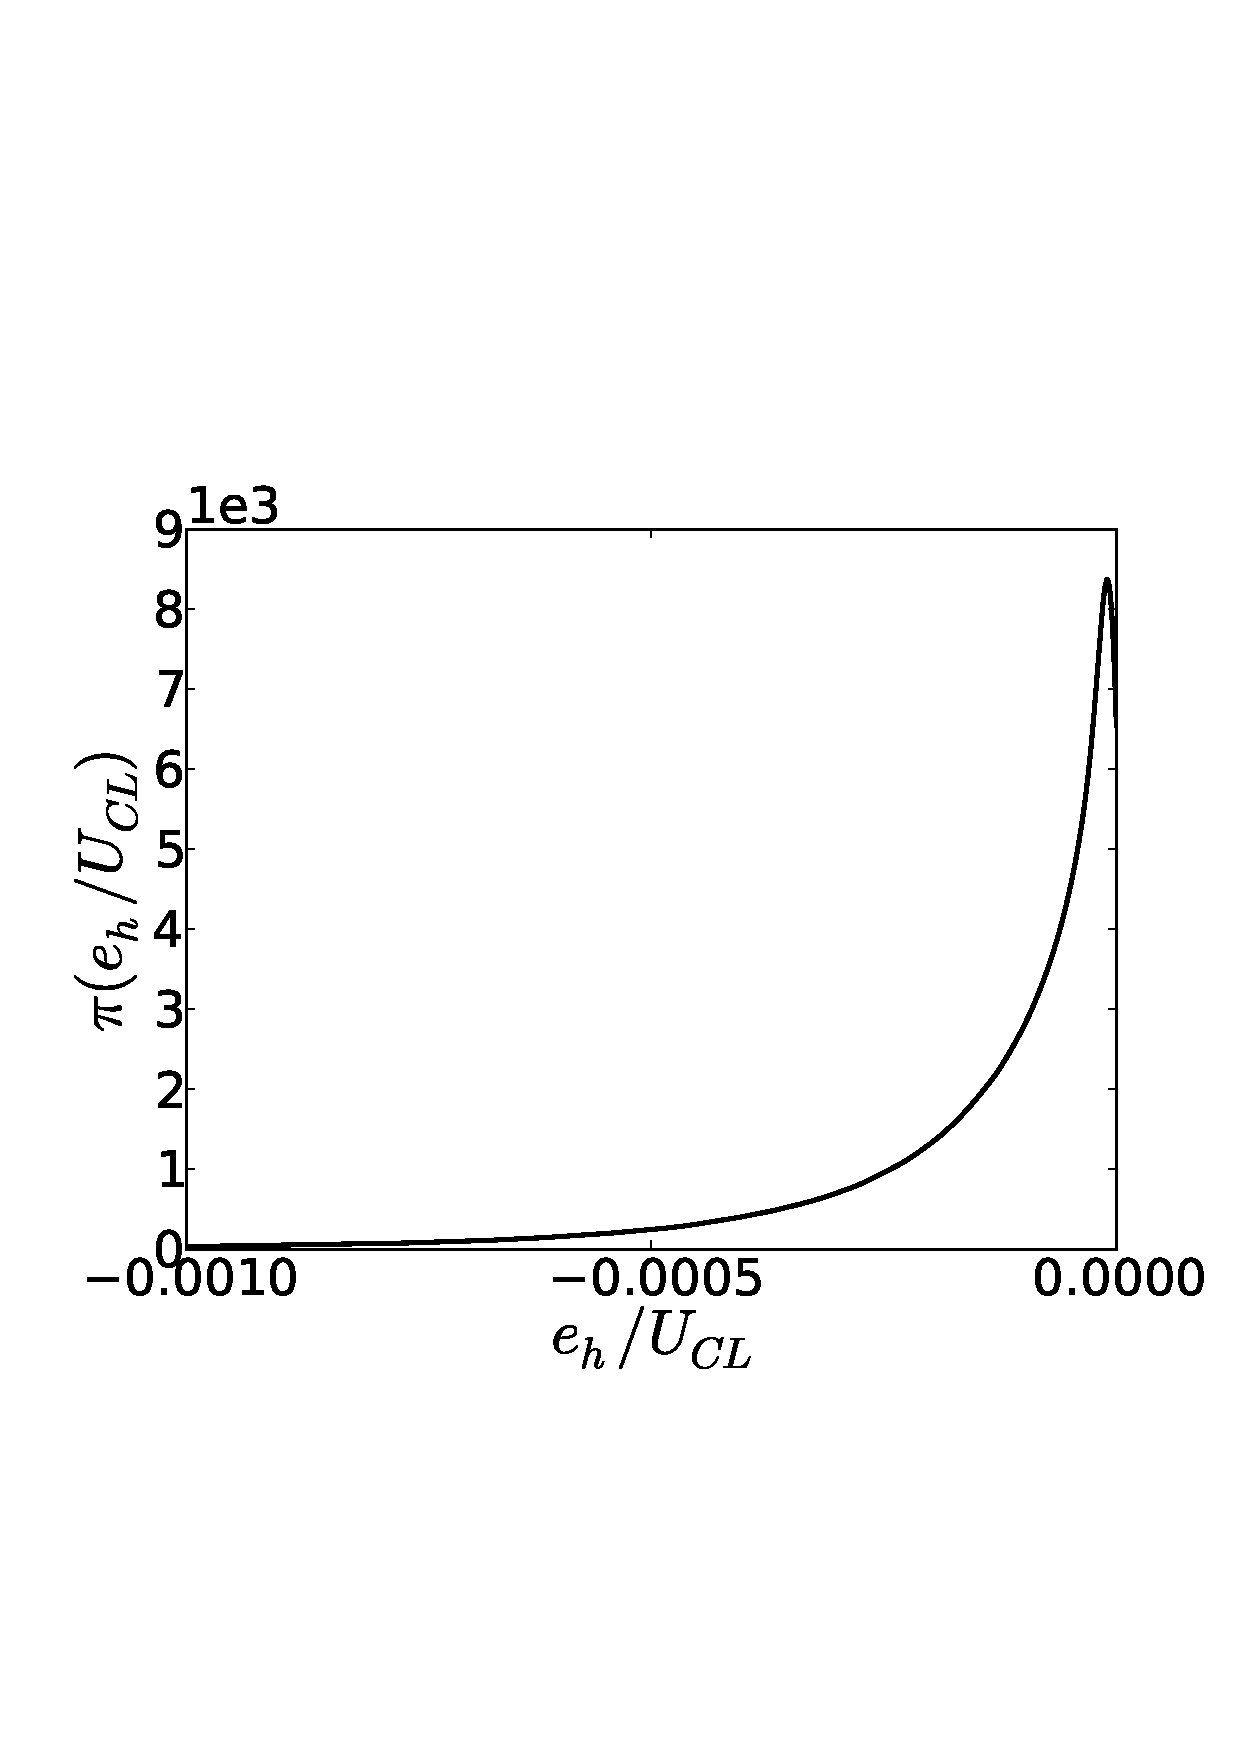
\includegraphics[width=0.99\linewidth]{cl_chp_disc_error_nominal.pdf}
    \end{center}
   \small 
   Discretization error, as computed by the calibrated model, for the
   centerline mean velocity on the nominal mesh. 
  \end{column}
  %
  \begin{column}{0.5\linewidth}
    \begin{center}
     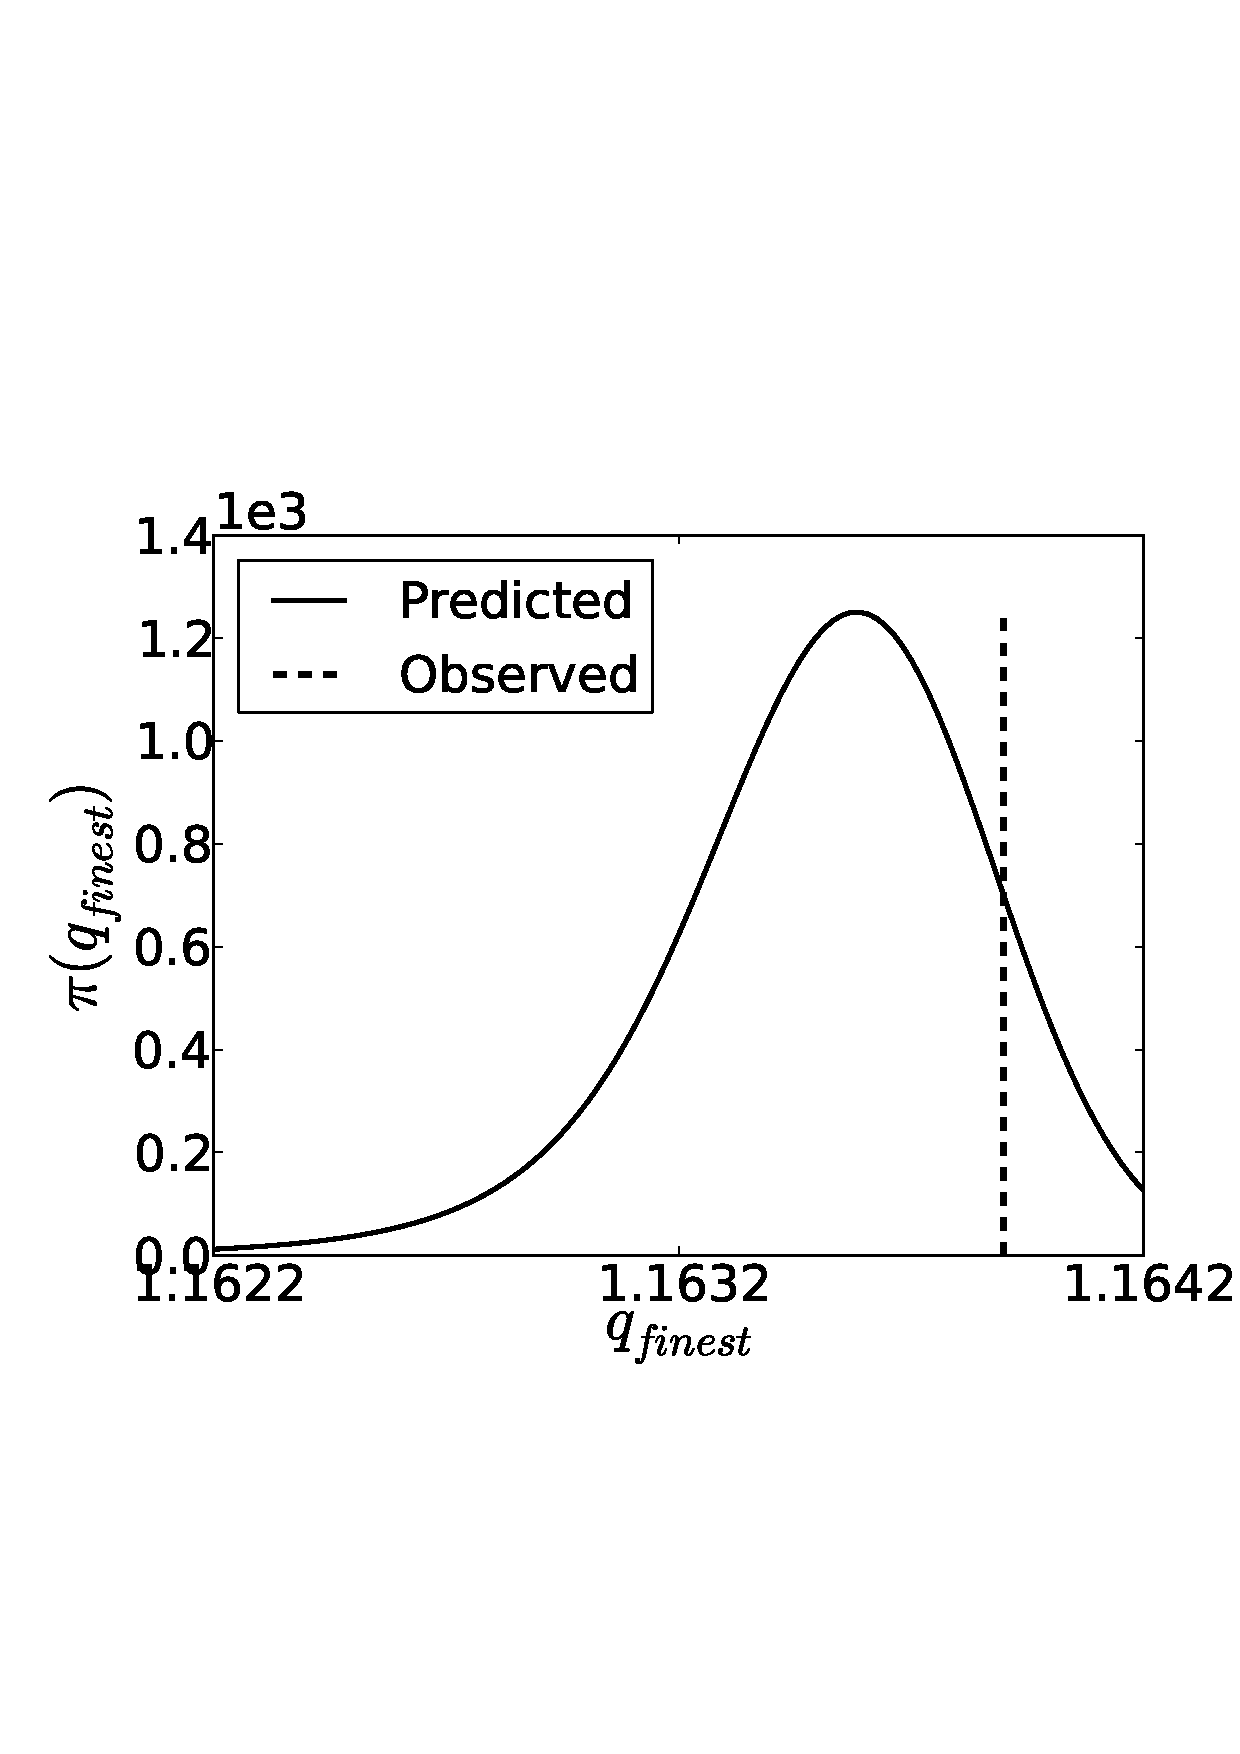
\includegraphics[width=0.99\linewidth]{cl_chp_qnext_post.pdf}
    \end{center}
   \small 
   PDF of the mean centerline velocity for the finest mesh predicted
   and the observed mean centerline velocity on the finest mesh. 
  \end{column}

\end{columns}
\end{frame}

%===============================================================================
\begin{frame}
\frametitle{Model Validation}
\begin{figure}[htp]
\centering
\begin{tabular}{ccc}
 Valid \subfloat[$\avg{u}$]{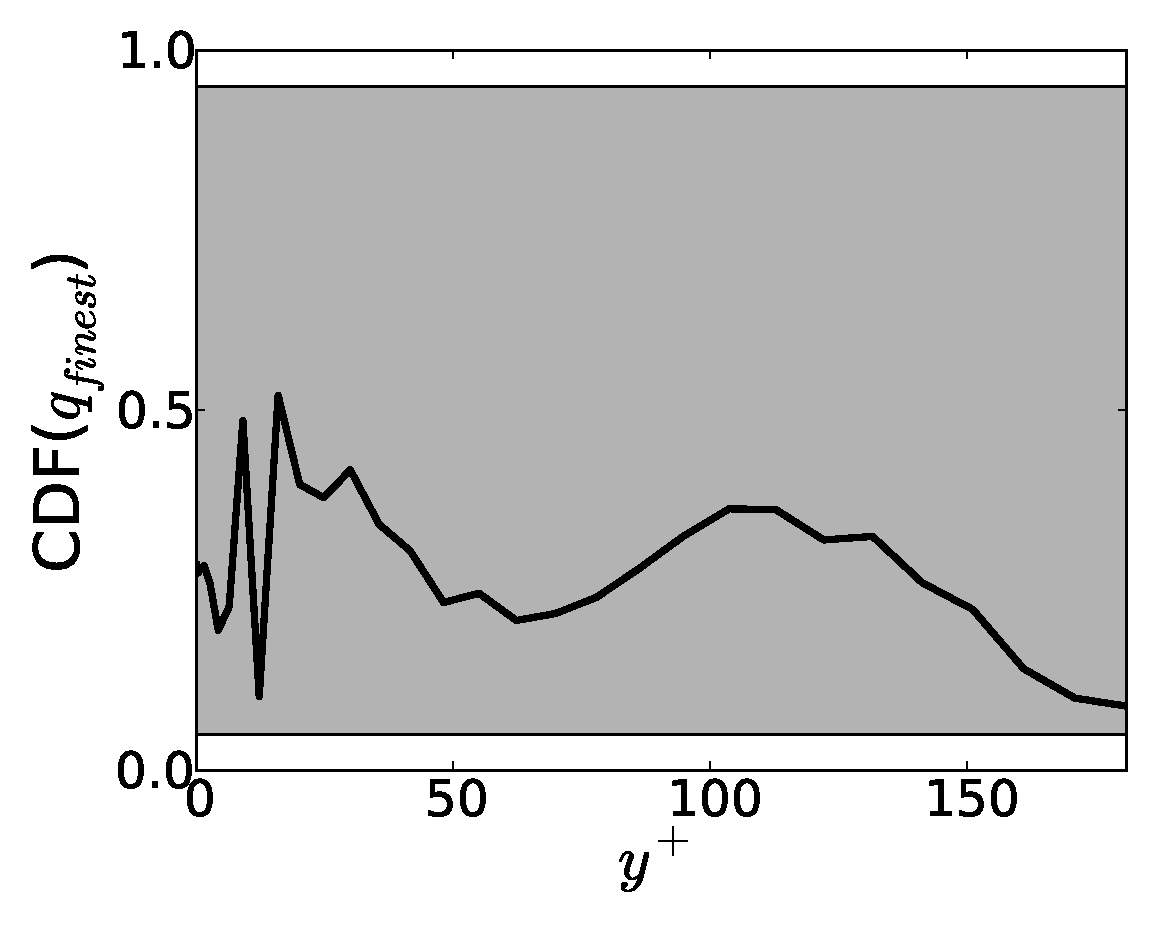
\includegraphics[width=0.26\linewidth]{mean_validation}}
 &
\subfloat[$\avg{v'v'}$]{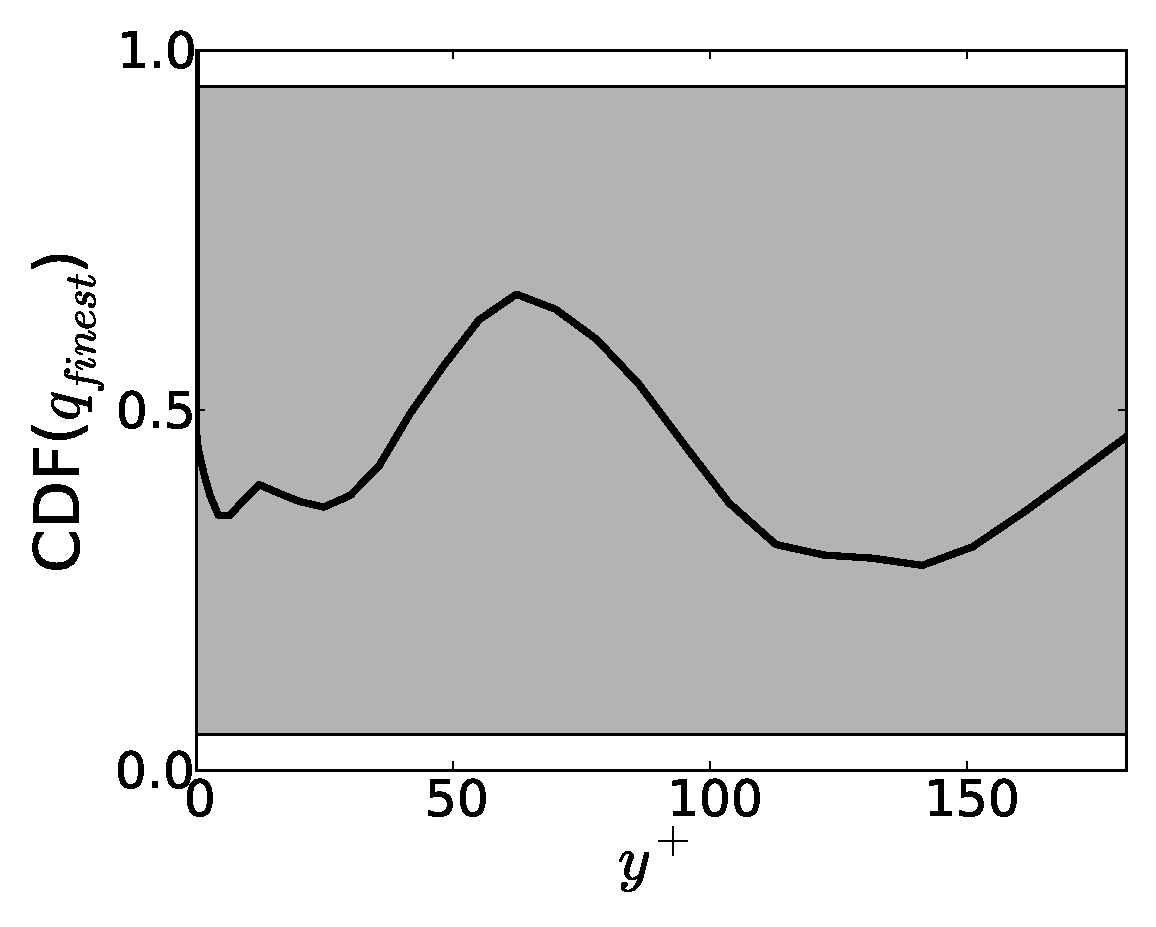
\includegraphics[width=0.26\linewidth]{vv_validation}}
     &
\subfloat[$\avg{w'w'}$]{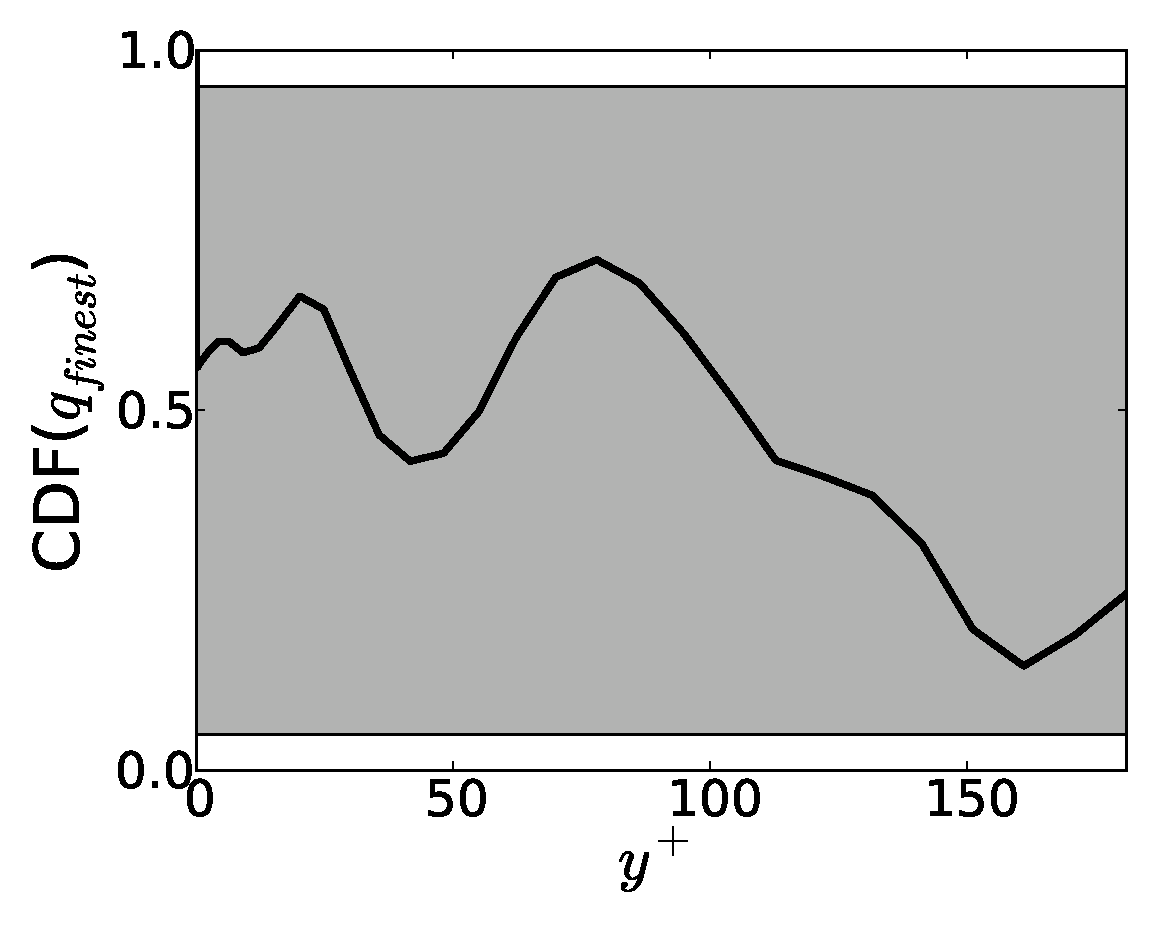
\includegraphics[width=0.26\linewidth]{ww_validation}} \\
Invalid \subfloat[$\avg{u'u'}$]{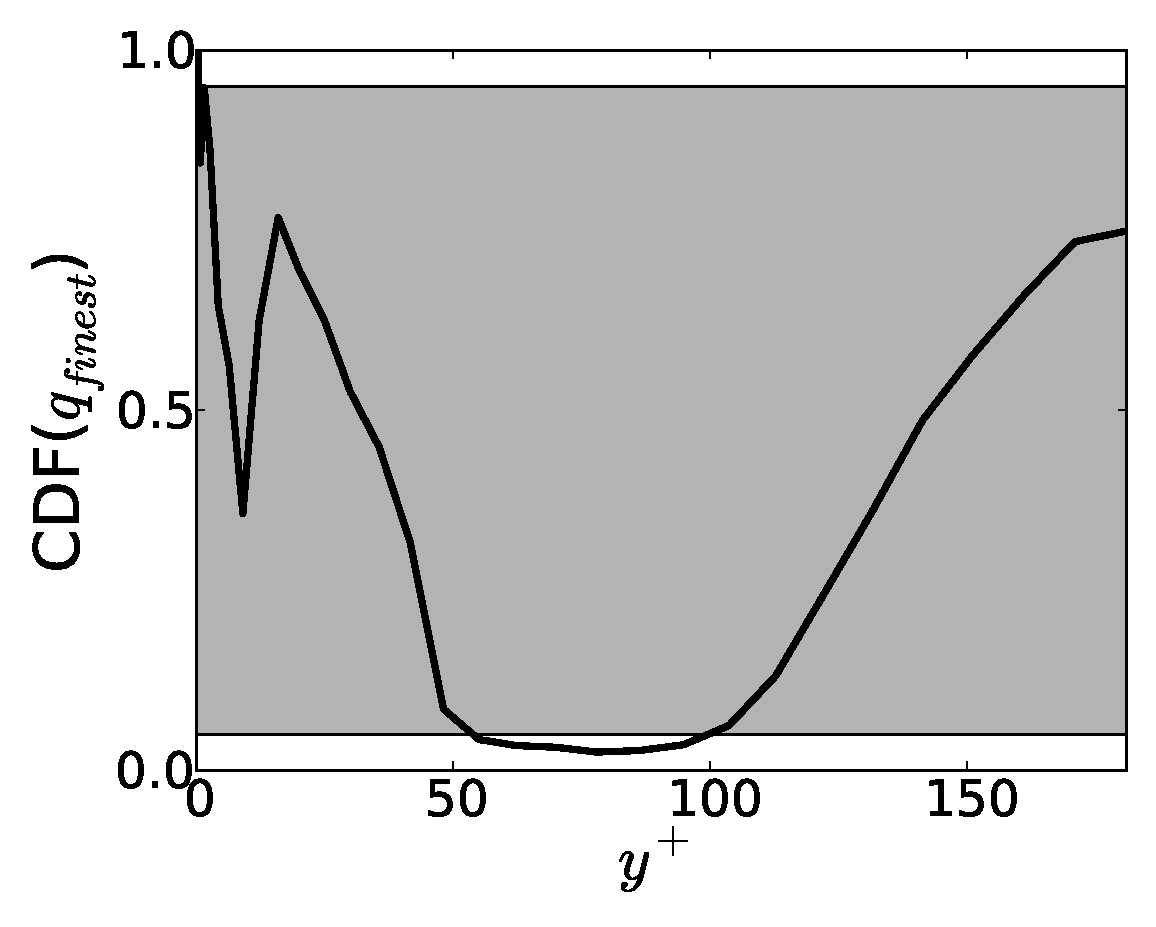
\includegraphics[width=0.26\linewidth]{uu_validation}}
 &
\subfloat[$\avg{\omega_y' \omega_y'}$]{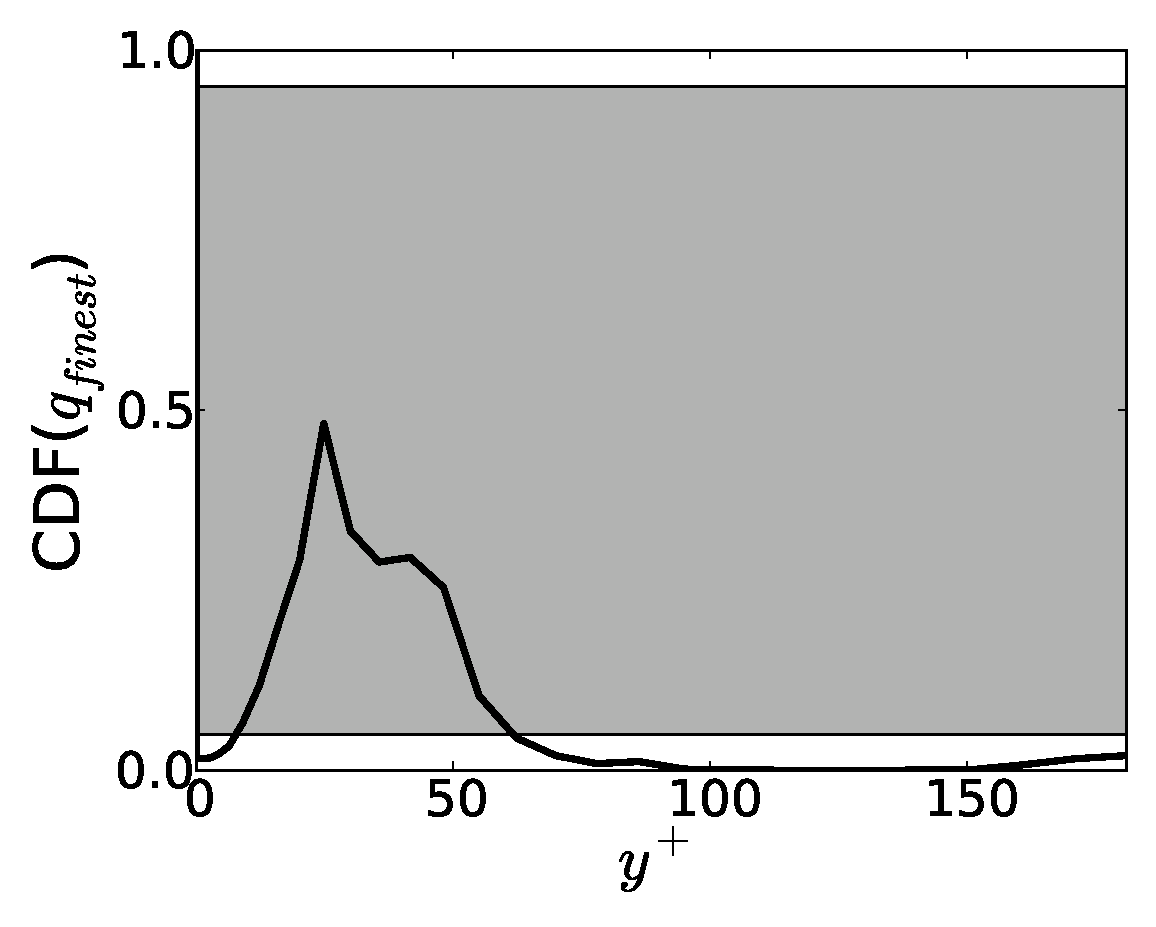
\includegraphics[width=0.26\linewidth]{omgy_validation}}
     &
\subfloat[$\avg{\omega_z' \omega_z'}$]{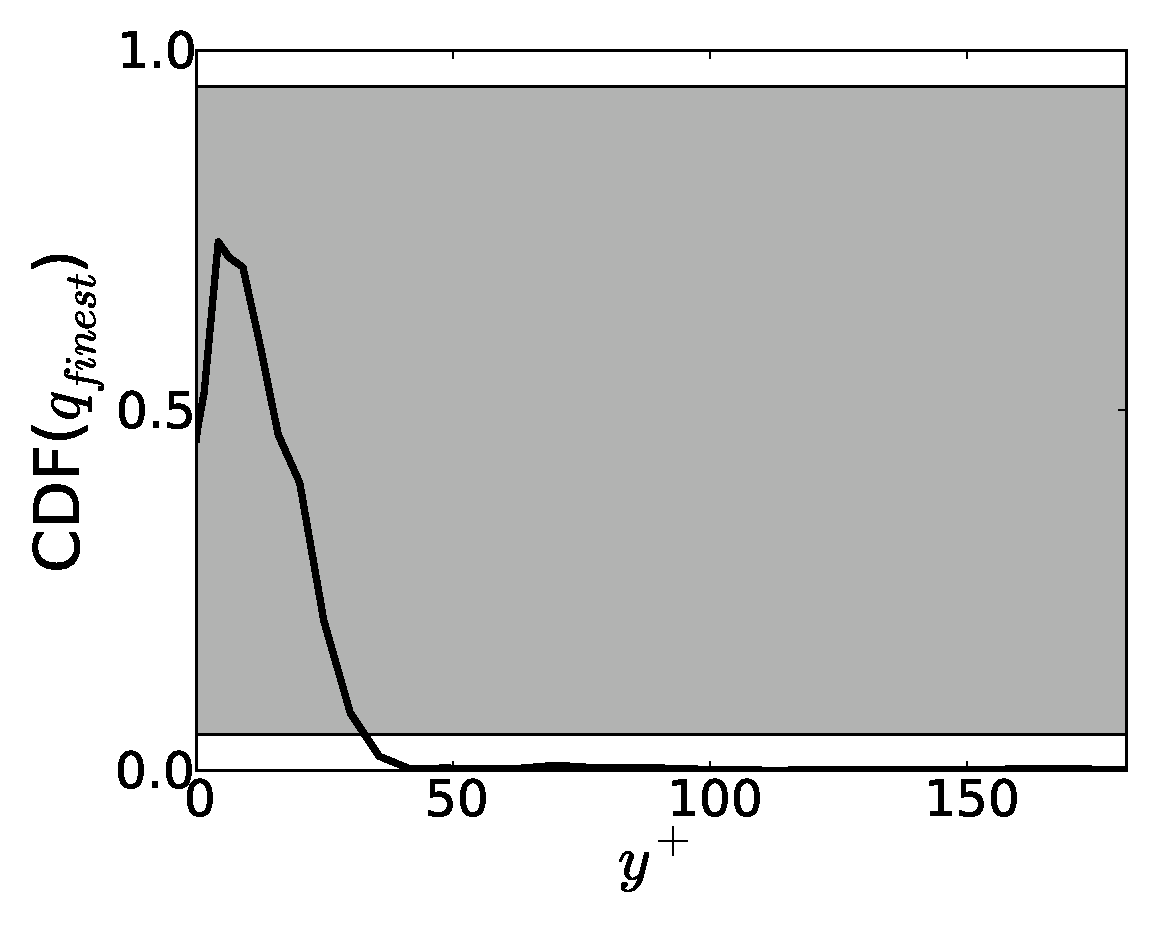
\includegraphics[width=0.26\linewidth]{omgz_validation}} \\
\end{tabular}
\end{figure}
\begin{itemize}
 \item Solid line is the computed value of the CDF at the observed value.
 \item Grey shows the 90\% credibility interval.
\end{itemize}
 
\end{frame}

%===============================================================================
% \begin{frame}
% \frametitle{Model (in)Validation}
% \begin{figure}[htp]
% \centering
% \begin{tabular}{ccc}
% \subfloat[$\avg{\omega_x' \omega_x'}$]{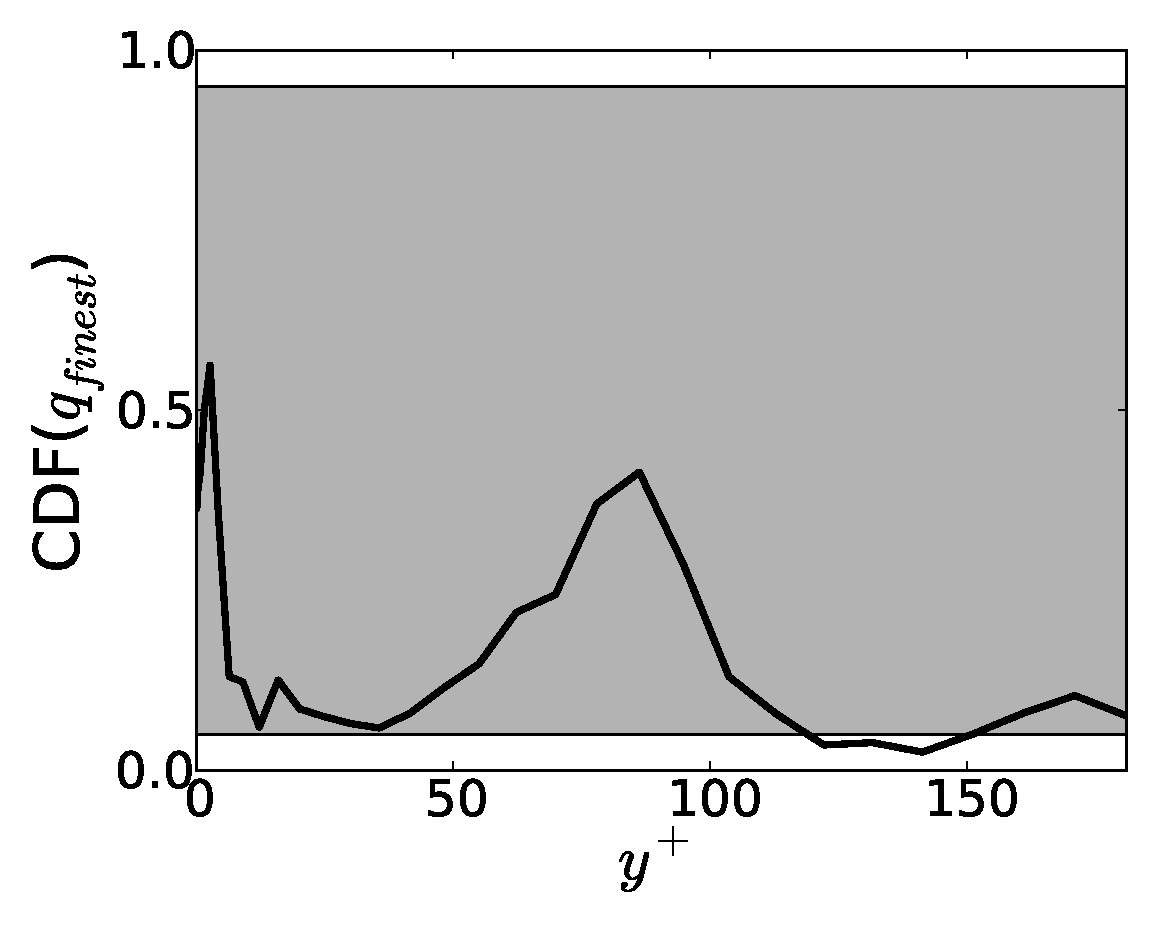
\includegraphics[width=0.3\linewidth]{omgx_validation}} &
% \subfloat[$\avg{\omega_y' \omega_y'}$]{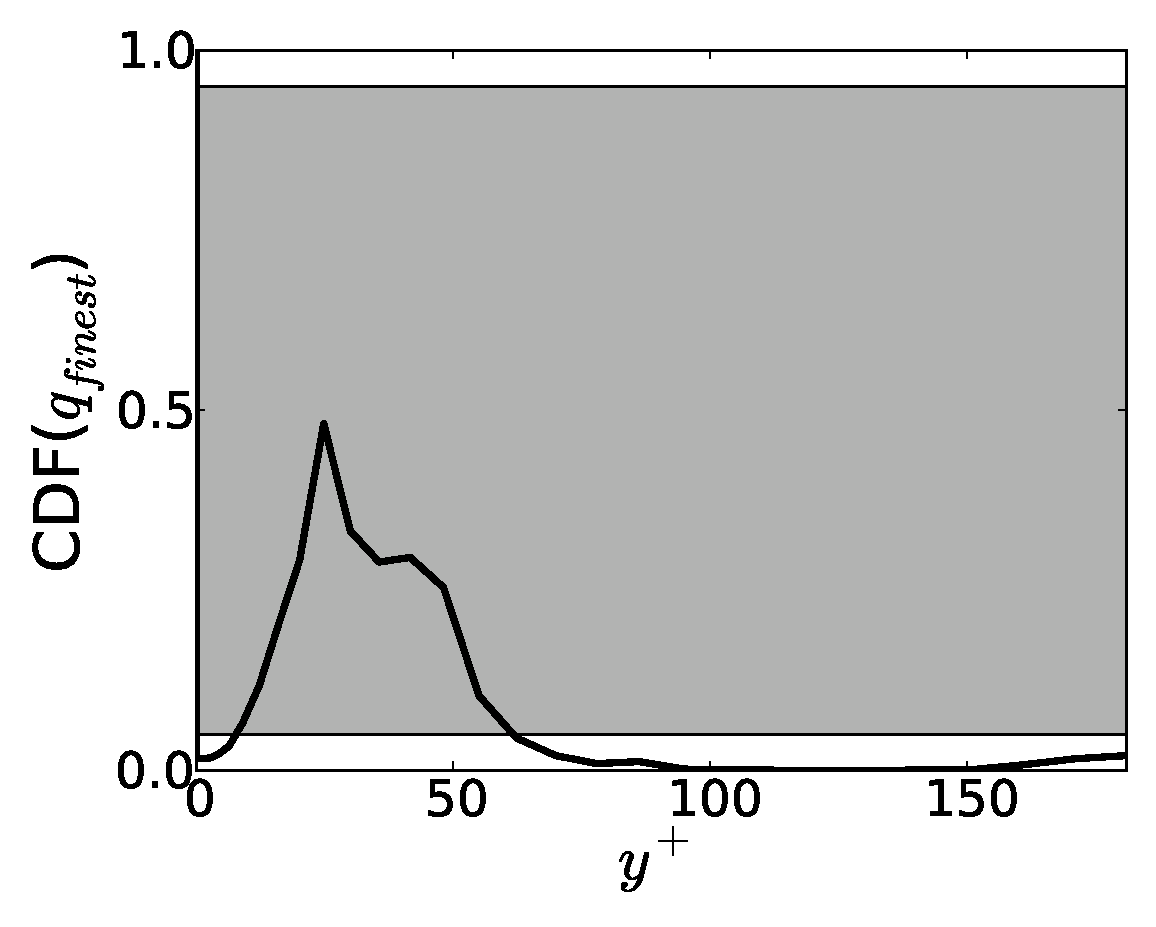
\includegraphics[width=0.3\linewidth]{omgy_validation}}
%      &
% \subfloat[$\avg{\omega_z' \omega_z'}$]{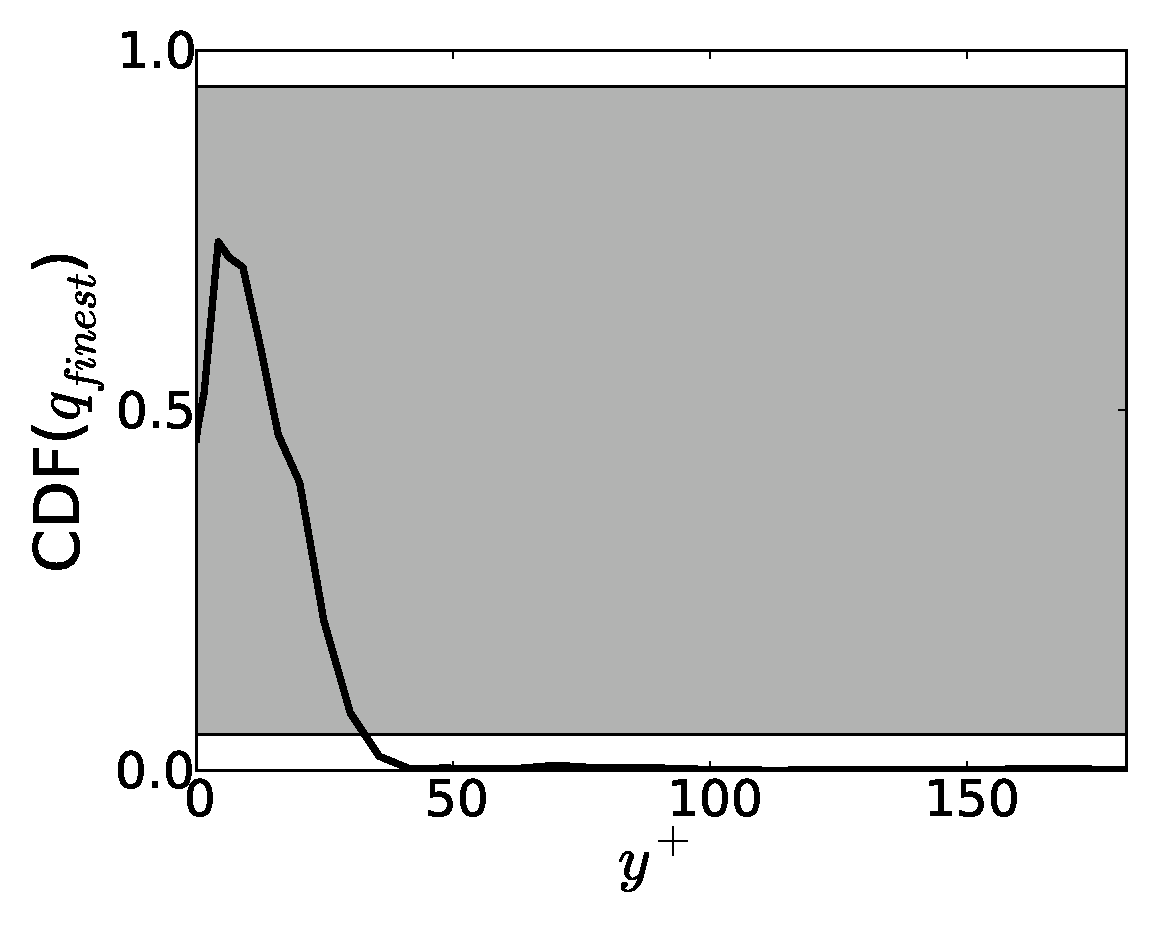
\includegraphics[width=0.3\linewidth]{omgz_validation}} \\
% \end{tabular}
% \end{figure}
% \begin{itemize}
%  \item Not converging monotonically with increasing mesh resolution.
%  \item The invalidity of the model does not imply that errors are large!
%        \begin{itemize}
% 	\item $\avg{u'u'} $ between nominal and finest mesh is less than
% 	      0.5\%
%        \end{itemize}
%        \end{itemize}
% \end{frame}

 \begin{frame}
   \frametitle{Conclusions}

   \begin{block}{}
    \center{Have a well validated day.} \\
    \center{nicholas.malaya@gmail.com}
    \end{block}

 \end{frame}

 
%===============================================================================
\end{document}
